%%%%%%%%%%%%%%%%%%%%%%%%%%%%%%%%%%%%%%%%
%12pt: grandezza carattere
%a4paper: formato a4
%openright: apre i capitoli a destra
%twoside: serve per fare un documento fronteretro
%report: stile tesi (oppure book)
\documentclass[12pt,a4paper,openright,twoside]{report}
\usepackage[utf8]{inputenc}
\usepackage[italian]{babel}
\usepackage{fancyhdr}
\usepackage{indentfirst}
\usepackage{graphicx}
\usepackage{newlfont}
\usepackage{textcomp}
\usepackage{subcaption}
%librerie matematiche
\usepackage{amssymb}
\usepackage{amsmath}
\usepackage{latexsym}
\usepackage{amsthm}
\usepackage{listings}
\usepackage{chngcntr}
\usepackage[chapter]{minted}


\oddsidemargin=30pt \evensidemargin=20pt%impostano i margini
\hyphenation{sil-la-ba-zio-ne pa-ren-te-si}

\usepackage[square, numbers, comma, sort&compress]{natbib} %Bibliografia
\usepackage{hyperref}
\usepackage{float}

\usepackage[pass]{geometry}

%comandi per l'impostazione della pagina, vedi il manuale della libreria fancyhdr per ulteriori delucidazioni
\pagestyle{fancy}\addtolength{\headwidth}{20pt}
\setlength{\headheight}{14.49998pt}
\renewcommand{\chaptermark}[1]{\markboth{\thechapter.\ #1}{}}
\renewcommand{\sectionmark}[1]{\markright{\thesection \ #1}{}}
\rhead[\fancyplain{}{\bfseries\leftmark}]{\fancyplain{}{\bfseries\thepage}}
\cfoot{}

\linespread{1.3} %comando per impostare l'interlinea

\renewcommand{\listingscaption}{Codice}
\renewcommand{\listoflistingscaption}{Elenco dei Codici}

%aggiunta per evitare che il link sbrodolino
\def\UrlBreaks{\do\/\do-}

\begin{document}
%%%%%%%%%%%%%%%%%%%%%%%%%%%%%%%%%%%%%%%%
% FRONTESPIZIO
\newgeometry{hmarginratio=1:1}
\begin{titlepage}
\begin{center}

\includegraphics[width=2.56in]{figures/logo/logo_unibo.png}\\
% {{\Large{\textsc{Alma Mater Studiorum $\cdot$ Universit\`a di
% Bologna}}}} \rule[0.1cm]{14.7cm}{0.1mm}
% \rule[0.5cm]{14.7cm}{0.6mm}
\vspace{5mm}
{\small{\bf SCUOLA DI INGEGNERIA E ARCHITETTURA\\
\vspace{2mm}
Dipartimento di Informatica -- Scienza e Ingegneria\\
\vspace{2mm}
Corso di Laurea in Ingegneria Informatica }}
%se Laurea Magistrale scrivere "Corso di Laurea Magistrale in Ingegneria Informatica"
\end{center}
\vspace{3,8mm}
\begin{center}
{\LARGE{\bf Cybersecurity e finanza:\\
\vspace{3,5mm}
analisi e studio delle conseguenze\\
\vspace{3,5mm}
finanziare degli attacchi informatici\\
\vspace{3,5mm}
sulle aziende\\
\vspace{3,5mm}}}
  
\end{center}
\vspace{9,5mm}
\par
\noindent
\begin{minipage}[t]{0.47\textwidth}
{\normalsize{\bf Relatore:\\
Prof. Dr. Marco Prandini\\

Correlatore:\\
Dr. Alessandro Vannini}}
\end{minipage}
\hfill
\begin{minipage}[t]{0.47\textwidth}\raggedleft
{\normalsize{\bf Presentata da:\\
Leonardo Ciacco}}
\end{minipage}
\vspace{7,5mm} % da aumentare a 10, 20 o 30 se non si inseriscono i correlatori
\begin{center}
{\normalsize{\bf Appello unico\\%inserire il numero dell'appello in cui ci si laurea CAPIRE
Anno Accademico 2024/2025}}%inserire l'anno accademico a cui si è iscritti
\end{center}
\end{titlepage}

\restoregeometry


%%%%%%%%%%%%%%%%%%%%%%%%%%%%%%%%%%%%%%%%
% ABSTRACT 
%\clearpage{\pagestyle{empty}\cleardoublepage}
%\pagenumbering{roman}
%\renewcommand{\abstractname}{Abstract}
%\phantomsection
%\addcontentsline{toc}{chapter}{Abstract}
%\begin{abstract}
%    Questo \`e l'abstract: un riassunto dell'introduzione di massimo 300 parole. Da scrivere alla fine.
%\end{abstract}


%%%%%%%%%%%%%%%%%%%%%%%%%%%%%%%%%%%%%%%%
% RINGRAZIAMENTI 
\clearpage{\pagestyle{empty}\cleardoublepage}
\chapter*{Ringraziamenti}
\phantomsection
\addcontentsline{toc}{chapter}{Ringraziamenti}
Grazie

\clearpage{\pagestyle{empty}\cleardoublepage}



%%%%%%%%%%%%%%%%%%%%%%%%%%%%%%%%%%%%%%%%
% INDICE 
\tableofcontents %crea l'indice
%imposta l'intestazione di pagina
\rhead[\fancyplain{}{\bfseries\leftmark}]{\fancyplain{}{\bfseries\thepage}}
\lhead[\fancyplain{}{\bfseries\thepage}]{\fancyplain{}{\bfseries
Indice}}



%%%%%%%%%%%%%%%%%%%%%%%%%%%%%%%%%%%%%%%%
% ELENCO DELLE FIGURE
\clearpage{\pagestyle{empty}\cleardoublepage}
\renewcommand{\listfigurename}{Elenco delle Figure}
\phantomsection
\addcontentsline{toc}{chapter}{Elenco delle Figure}
\listoffigures %crea l'elenco delle figure



%%%%%%%%%%%%%%%%%%%%%%%%%%%%%%%%%%%%%%%%
% ELENCO DELLE TABELLE
\clearpage{\pagestyle{empty}\cleardoublepage}
\renewcommand{\listtablename}{Elenco delle Tabelle}
\phantomsection
\addcontentsline{toc}{chapter}{Elenco delle Tabelle}
\listoftables %crea l'elenco delle tabelle



%%%%%%%%%%%%%%%%%%%%%%%%%%%%%%%%%%%%%%%%
% INTRODUZIONE
\clearpage{\pagestyle{empty}\cleardoublepage}
\chapter{Introduzione} 
\lhead[\fancyplain{}{\bfseries\thepage}]{\fancyplain{}{\bfseries\rightmark}}
\pagenumbering{arabic} %mette i numeri arabi
Il pericolo degli attacchi informatici \`e tristemente noto, ci\`o che viene spesso trascurato \`e l'impatto concreto e 
misurabile sui piani econimico e finanziario. Oltre le spese di ripristino concorrono al danno concreto anche perdita di 
fiducia, valore di mercato e stabilit\`a dell'organizzazione.\\

Tramite l'analisi di 15 casi di studio, questo elaborato si propone di fornire un dato reale che aiuti a diffondere una 
maggiore consapevolezza in materia. Nel capitolo \ref{chap:artState} vi \`e una analisi dello Stato dell'Arte per 
comprendere il panorama degli attacchi informatici. A seguire verranno sviscerati i singoli casi nel capitolo 
\ref{chap:attacks}, per poi metterli a confronto e interpretare i dati ottenuti nel capitolo \ref{chap:analisys}.\\ 

\clearpage{\pagestyle{empty}\cleardoublepage}



%%%%%%%%%%%%%%%%%%%%%%%%%%%%%%%%%%%%%%%%
% STATO DELL'ARTE
\chapter{Analisi dello stato dell'arte e del contesto}\label{chap:artState}
Il presente capitolo mira a fornire le informazioni fondamentali, necessarie a comprendere i futuri sviluppi. A questo scopo sono definiti alcuni concetti chiave in ambito di sicurezza informatica:
\begin{itemize}
    \item rischio
    \item sicurezza
    \item minaccia
    \item vulnerabilit\`a
    \item attacco
\end{itemize}
Con \textbf{rischio} si intende la possibilit\`a che azioni umane o eventi  abbiano un impatto su ci\`o a cui \`e attribuito valore. \`E quindi corretto affermare che si tratta di una grandezza, e come tale \`e quantificabile, \`e infatti direttamente proporzionale alla probabilit\`a di avvenimento e all'impatto che avrebbe sui beni colpiti. La valutazione del rischio, mirata alla sua gestione e controllo, parte dalla stima quanto pi\`u accurata di queste due variabili.\\
\\
La \textbf{sicurezza} \`e il processo di contenimento del rischio che consiste essenzialmente nella cura di tre propriet\`a fondamentali: riservatezza (inaccessibilit\`a delle informazioni a chi non ha il permesso di consultarle), integrit\`a (garanzia di correttezza delle informazioni) e disponibilit\`a (possibilit\`a di accesso e utilizzo delle informazioni e i servizi offerti).\\
\\
La \textbf{minaccia} consiste nella potenziale compromissione di una o pi\`u delle propriet\`a sopracitate, e, da concetto astratto, si concretizza in un \textbf{attacco}: azione di sfruttamento (\textit{exploit}) delle vulnerabilit\`a di un sistema\\

\section{Tipologie di attacco}
ENISA (Agenzia dell'Unione Europea per la Cybersicurezza) raggruppa gli attacchi informatici in otto categorie principali.\cite{enisa_threat_landscape}
\subsection{Ransomware}
Definito come un tipo d attacco in cui gli attori coinvolti prendono il controllo di un bene del bersaglio e chiedono un riscatto (in inglese \textit{ransom}) in cambio della restituzione. \`E un tipo di attacco  generalmente attuato per scopi economici, ma, essendo anche uno dei pi\`u diffusi evolve rapidamente, sia dal punto di vista delle tecniche di estorsione che degli obiettivi.\\

\subsection{Malware}
Si tratta di un termine ombrello: descrive tutti i \textit{software} o \textit{firmware} con lo scopo di eseguire un processo non autorizzato sulla macchina ospitante il cui risultato \`e la compromissione di una delle tre propiet\`a della sicurezza.\\

\subsection{Ingegneria sociale}
Gli attacchi tramite ingegneria sociale si distinguono per lo sfruttamento della vulnerabilit\`a derivata dall'errore umano. Consistono nel mettere in atto tecniche di manipolazione per indurre chi coinvolto nella gestione dei beni bersaglio a rilasciare informazioni sensibili, concedere permessi 
apparentemente innocui, visitare siti, aprire file, documenti o e-mail con contenuto malevolo. Un esempio pu\`o essere il \textit{phishing}, in cui si cerca di indurre la vittima ad aprire un link ad un sito che scarica un \textit{malware}.\\
L'ingegneria sociale \`e spesso protagonista delle fasi iniziali di un attacco, ma questo non esclude che possa essere impiegata in stadi pi\`u avanzati. Ad esempio, \`e chiamata BEC (\textit{Business E-mail Compromise}) l'intrusione tramite vecchie credenziali aziendali che le sfrutta, fingendosi parte dell'organizzazione, per ottenere dagli ex colleghi informazioni, denaro, o risorse altrimenti inaccessibili.\cite{IBM_BEC}\\

\subsection{Violazioni di dati}
Tecnicamente vi ci si riferisce con i termini inglesi \textit{data breach} o \textit{data leak}.  
Da definizione del GDPR, per violazione dei dati personali intendiamo la ``violazione di sicurezza che comporta accidentalmente o in modo illecito la distruzione, la perdita, la modifica, la divulgazione non autorizzata o l'accesso ai dati personali trasmessi, conservati o comunque trattati'' (articolo 4.12 GDPR). \\
La differenza risiede nell'intenzionalità: il \textit{breach} \`e un attacco con l'esplicito obiettivo di ottenere o diffondere dati sensibili o protetti, il \textit{leak} è originato da un errore che porta ad una indesiderata perdita o messa a disposizione di dati sensibili. \\

\subsection{Minacce alla disponibilit\`a: DoS}
Per definizione, un DDoS (\textit{Distriubuted Denial of Service}), si verifica come risultato di un attacco che mira a rendere inaccessibili servizi o risorse tramite, per esempio, uno sproporzionato volume di richieste che sovraccarica i componenti della struttura attaccata.
In questo caso quindi l'obiettivo risiede nella semplice interruzione dei servizi erogati.\\

\subsection{Minacce alla disponibilit\`a: minacce ad Internet}
Alla base della disponibilit\`a dei servizi nella societ\`a dell'informazione vi \`e l'infrastruttura di internet, che se subisce guasti distribuiti pu\`o comprometterne quasi completamente l'erogazione. Sebbene sia un'ipotesi remota,  blackout, disastri naturali, interruzione forzata da parte del governo o attacchi su larga scala rappresentano una minaccia concreta che non pu\`o essere sottovalutata.\\

\subsection{Manipolazione delle informazioni}
Si chiama \textit{Foreign Information Manipulation and Interference}, abbreviato in FIMI, l'insieme di strategie di manipolazione dell'opinione pubblica da parte di enti, governativi e non, volte ad inserirsi nel dibattito in maniera massiccia e organizzata. Ci\`o mina i processi decisionali democratici tramite campagne di disinformazione e narrazioni precostruite.\\
\subsection{Attacchi alla catena di fornitura}
Pi\`u comunemente  chiamati \textit{supply chain attacks}, sono attacchi che sfruttano la fiducia riposta nei servizi offerti da partner commerciali o fornitori, colpendo l'obiettivo indirettamente tramite la compromissione di un fornitore legittimo.\\
Pi\`u formalmente, un attacco \`e considerato in parte di natura \textit{supply chain} se consiste nella combinazione di almeno due attacchi coordinati. Perch\'e sia identificato come tale, devono infatti essere bersaglio sia l'obiettivo intermedio, fornitore, che l'obiettivo finale, naturalmente vulnerabile nei confronti chi valuta fonte sicura. \\
%SolarWinds
%was one of the first revelations of this kind of attack and showed the potential impact of supply chain attacks. It was observed that threat actors are continuing to feed on this source to conduct their operations and gain a
%foothold within organisations, to benefit from the widespread impact and large victim base of such attacks



\section{Contesto economico}
Con l'esponenziale crescita ed espansione dei mezzi di informazione, crescono anche i mercati illeciti, precisamente il costo del cybercrimine era di \$3 trilioni nel 2015 e, si stima, toccher\`a i \$10.5 trilioni durante il 2025\cite{cybercrime_magazine}. Se fosse il PIL di uno stato sarebbe sicuramente tra i primi cinque al mondo.\\
In un panorama di questo tipo le aziende quotate in borsa, soprattutto le pi\`u in risalto come quelle in indici come S\&P500, sono un bersaglio estremamente appetibile per chiunque abbia i mezzi e l'intenzione di danneggiarle in quanto:
\begin{itemize}
  \setlength{\itemsep}{0pt}
  \setlength{\parskip}{0pt}       
  \renewcommand{\labelitemi}{\textbf{--}} 
  \item sono in possesso di grandi quantit\`a di \textbf{dati sensibili}: questo sopratutto se si tratta di grandi aziende o se specializzate nel settore, ma chiaramente, se l'obiettivo \`e il furto di informazioni, un'alta concentrazione delle stesse agisce da incentivo;
  \item sono facilmente \textbf{valutabili}: per eseguire un attacco \textit{ransomware} occorre anche commisurare la richiesta di riscatto al valore del bene per l'azienda e alla sua disponibilit\`a economica, i bilanci pubblici offrono quindi una fonte di informazioni  preziosa;
  \item se attaccate, hanno \textbf{reazioni} spesso \textbf{prevedibili}: secondo un rapporto di Accenture del 2010 \cite{accenture2010}, le aziende che subiscono un attacco sperimentano un calo di prezzo delle azioni che si aggira solitamente intorno al 5\%, rivelando come l'attacco potrebbe essere sfruttato ulteriormente come strumento di controllo illecito del mercato per trarre  ulteriori profitti collaterali.
\end{itemize}
Solo nel 2023, il 21\% selle aziende in S\&P500 hanno subito un \textit{breach}\cite{SecurityScorecard_SP500}.\\
\\
Inoltre, i danni connessi agli attacchi sono ugualmente preoccupanti, tra questi:
\begin{itemize}
  \setlength{\itemsep}{0pt}   
  \setlength{\parskip}{0pt}       
  \renewcommand{\labelitemi}{\textbf{--}}  
  \item ripercussioni legali;
  \item perdita di fiducia di clienti ed investitori.
\end{itemize}
Un attacco pu\`o avere diversi scopi, di cui, primo tra tutti, quello economico, ma il panorama degli attacchi \`e vasto, e pensare di non poter essere bersagli appetibili \`e un errore pericoloso per l'azienda e chiunque vi sia collegato. \cite{enisa_threat_landscape}\\
A fronte di ci\`o risulta gi\`a evidente quanto sia necessario essere a conoscenza dell'entit\`a del rischio di un attacco informatico che, vista anche la forte crescita e diffusione, non pu\`o essere ignorata. Va quindi sviluppato un piano d'azione dettagliato e coerente con la valutazione dei beni a rischio, finanziato adeguatamente.\\

\section{Metodologia}
Lo studio si propone di analizzare 15 casi di attacchi informatici, con focus sulle ripercussioni che questi hanno avuto sull'azienda.\\
Gli attacchi sono di vario tipo, e sono avvenuti tra il 2011 e il 2024 l'analisi \`e condotta con l'obiettivo di individuare un trend e ,in generale, valutare la minaccia crescente del cybercrimine.\\  
\clearpage{\pagestyle{empty}\cleardoublepage}



%%%%%%%%%%%%%%%%%%%%%%%%%%%%%%%%%%%%%%%%
% Attacchi e conseguenze finanziarie
\chapter{Attacchi e conseguenze finanziarie}\label{chap:attacks}
Nota: la maggior parte dei grafici proviene da \href{https://www.macrotrends.net/}{macrotrends}.

\section{Sony Playstation Network (2011)}
\subsection{Descrizione}
Il 20 aprile 2011 Sony dichiar\`o che tra il 17 e il 19 dello stesso mese avvenne un importante \textit{data breach} , a seguito di cui disabilit\`o per una settimana il servizio online Playstation Network. L'attacco port\`o al furto di dati sensibili riguardanti 77 milioni di account\cite{Sony_PNT_guardian}\cite{Sony_pnt}.\\
\subsection{Impatto diretto}
Sony sub\`i diverse conseguenze legali, che unite agli obblighi di miglioramento della sicurezza, si stima ebbero un costo complessivo di \$171 milioni.\\
\subsection{Impatto indiretto}
Come si pu\`ovedere dalla figura \ref{fig:pnt1} e nelle fonti \cite{Sony_pnt} la compagnia sub\`i, nei primi giorni, un calo del valore delle azioni  superiore al 3\%.\\

\begin{figure}[H] 
\begin{center} 
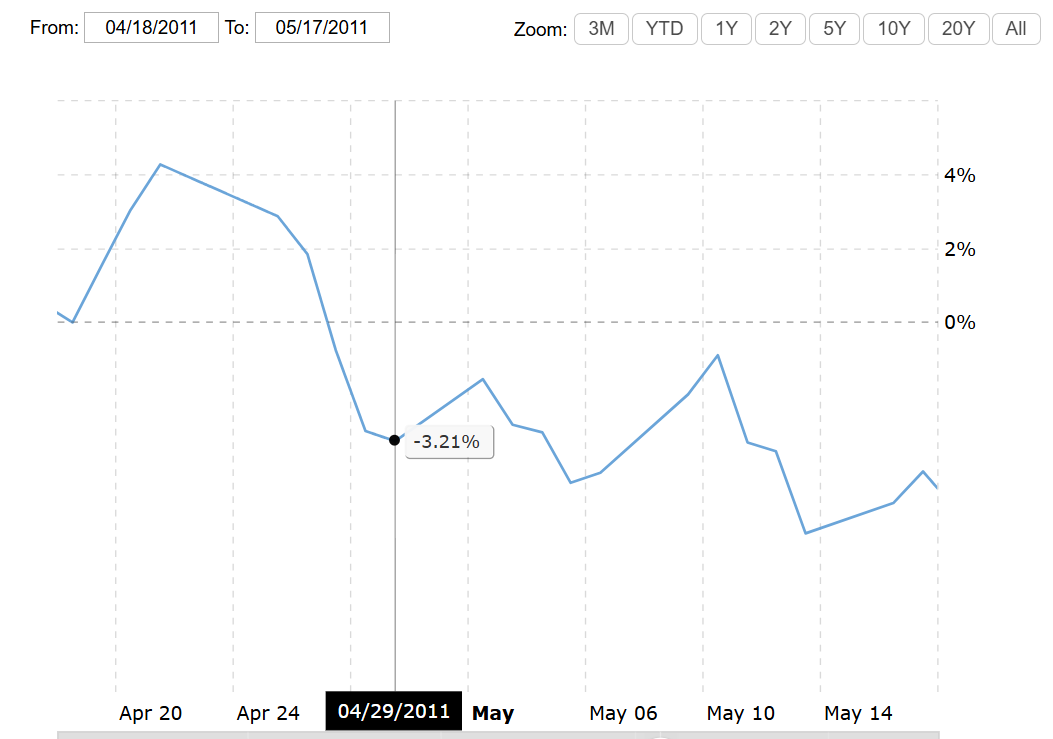
\includegraphics[width=10cm]{figures/sony_2011_shortTerm.png} 
\caption[Grafico Sony PSN short]{Impatto a breve termine Sony Playstation Network Outage}\label{fig:pnt1}
\end{center}
\end{figure}

A seguito inizia un periodo di contrazione che, possiamo osservare, porta i valori delle azioni da pi\`u di \$5 nel periodo antecedente alla crisi, fino a scendere sotto i \$2 nel 2013 (adjusted). \\Associare la parabola discendente esclusivamente all'attacco \`e forse esagerato, ci\`o non toglie che si tratti sicuramente di un fattore rilevante.\\ 

\begin{figure}[H] 
\begin{center} 
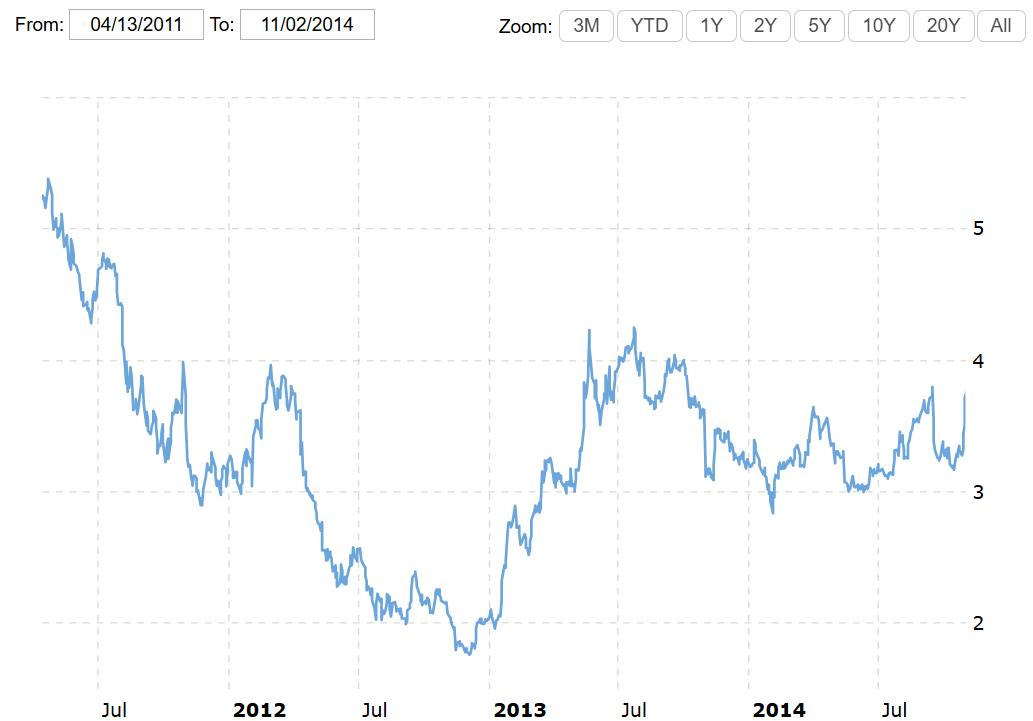
\includegraphics[width=10cm]{figures/sony_2011_longTerm.png} 
\caption[Grafico Sony PSN long]{Impatto a lungo termine Sony Playstation Network Outage}\label{fig:pnt2}
\end{center}
\end{figure}


\subsection{Note}
Le comunicazioni furono tardive e poco precise, gli azionisti ebbero notizia del motivo per cui Playstation Network era disabilitato solo 7 giorni dopo, e i comunicati ai clienti non furono da meno, alimentando malcontento e sfiducia nelle capacit\`a dell'azienda\cite{Sony_pnt}.
\section{Target (2013)}
\subsection{Descrizione}
Il caso di \textit{data breach} affrontato riguarda l'azienda di distribuzione Target, seconda negli Stati Uniti solamente a Walmart, e l'attacco che si \`e concluso con il furto di  informazioni, comprese informazioni di pagamento e carte di credito, di 70 milioni di clienti.\\
Prime avvisaglie dell'ingresso di un malware nella rete arrivano il 30 novembre 2013, probabilmente avvenuto per via dell'utilizzo di password troppo semplici nei server aziendali, ma \`e dal 12 dicembre che, in seguito alla notifica del Dipartimento di Giustizia, iniziano le indagini congiunte. Verificatane l'entit\`a, la notizia viene resa di dominio pubblico il 19 dicembre 2013\cite{Target}.\\
\subsection{Impatto diretto}
Da quanto dichiarato nei bilanci SEC (\textit{Securities and Exchange Commission}), le spese dirette, tolti \$90 milioni coperti da assicurazione, ammontano a \$200 milioni\cite{Target}.
\subsection{Impatto indiretto}
Sebbene nei giorni immediatamente successivi ci sia stato un picco verso il basso di -2.2\% \ref{fig:tgt1}, con momenti di ulteriore discesa, e sebbene l'andamento sia stato praticamente neutro per un anno, dalla fine del 2014 l'azienda ha recuperato parte della crescita inespressa fino ad allora \ref{fig:tgt2}. Ad aiutare \`e stata l'ottima immagine che ha nei confronti dei clienti e la fiducia dei pi\`u affezionati ad un marchio decisamente forte.\\
\begin{figure}[H] 
\begin{center} 
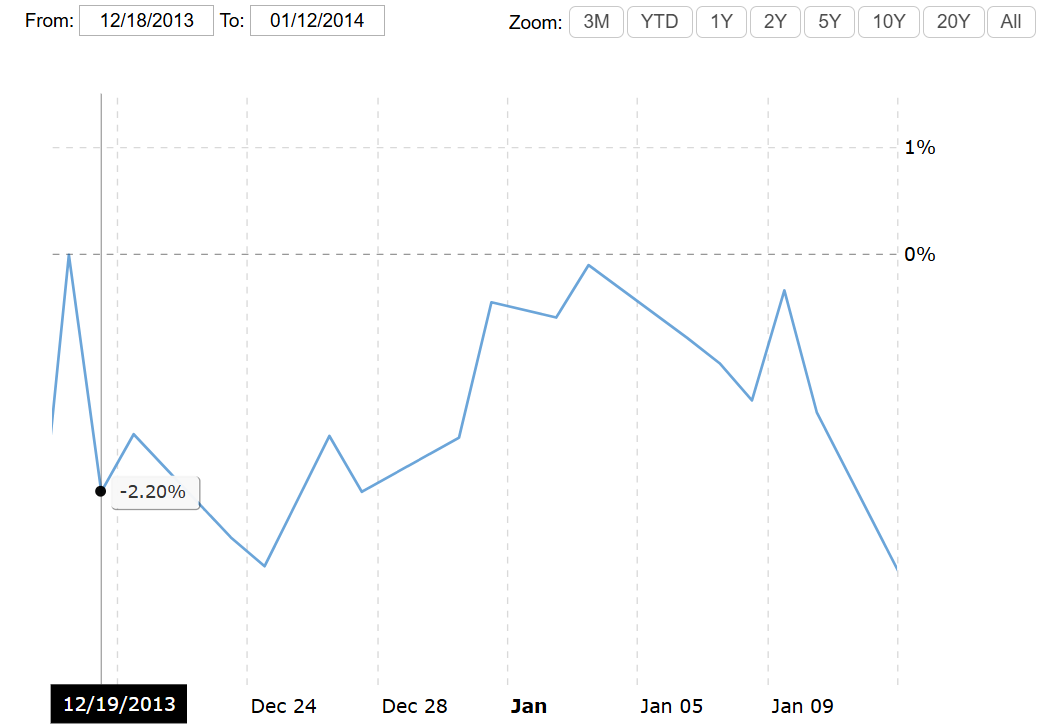
\includegraphics[width=10cm]{figures/target_short.png} 
\caption[Grafico Target short]{Impatto a breve termine Target data breach}\label{fig:tgt1}
\end{center}
\end{figure}
\begin{figure}[H]
\begin{center} 
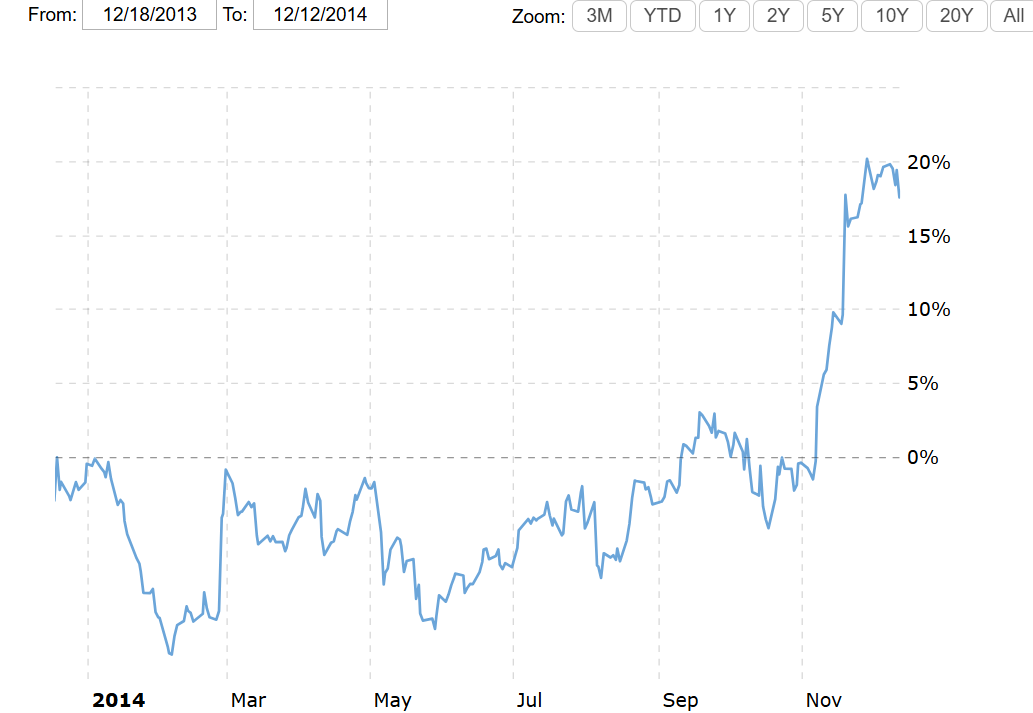
\includegraphics[width=10cm]{figures/target_long.png} 
\caption[Grafico Target long]{Impatto a lungo termine Target data breach}\label{fig:tgt2}
\end{center}
\end{figure}

\section{Sony Pictures (2014)}

\subsection{Descrizione}
Sony Pictures Entertainment viene colpito da un attacco informatico di tipo \textit{data breach} a fine novembre 2014, vengono rilasciati 40GB di informazioni che, a detta degli attaccanti, fanno parte di un furto del volume di 100TB. Dentro vi troviamo pi\`u di 6800 dati salariali dei dipendenti, e anticipazioni riguardanti serie TV e film ancora in fase di produzione\cite{SonyPic_buzzfeed}.\\
\subsection{Impatto diretto}
L'azienda dichiara, nel bilancio SEC per aziende estere, di aver speso \$41 milioni per spese investigative e correlate all'attacco e che dovr\`a sostenere spese legali nei confronti di dipendenti ed ex dipendenti\cite{SonyPic_20F_report}. A fine anno trover\`a un accordo per stanziare \$8 milioni di risarcimento.\\

\subsection{Impatto indiretto}
Come notiamo in figura \ref{fig:sPic1}, l'attacco ha progressivamente portato le azioni dell'intero gruppo Sony a -5\% e fino a toccare il -10\% a met\`a dicembre, sopratutto per l'importante risonanza mediatica del caso e il fatto che fosse la seconda volta in pochi anni che il nome della compagnia era accostato a casi di furto di informazioni.\\
\begin{figure}[H] 
\begin{center} 
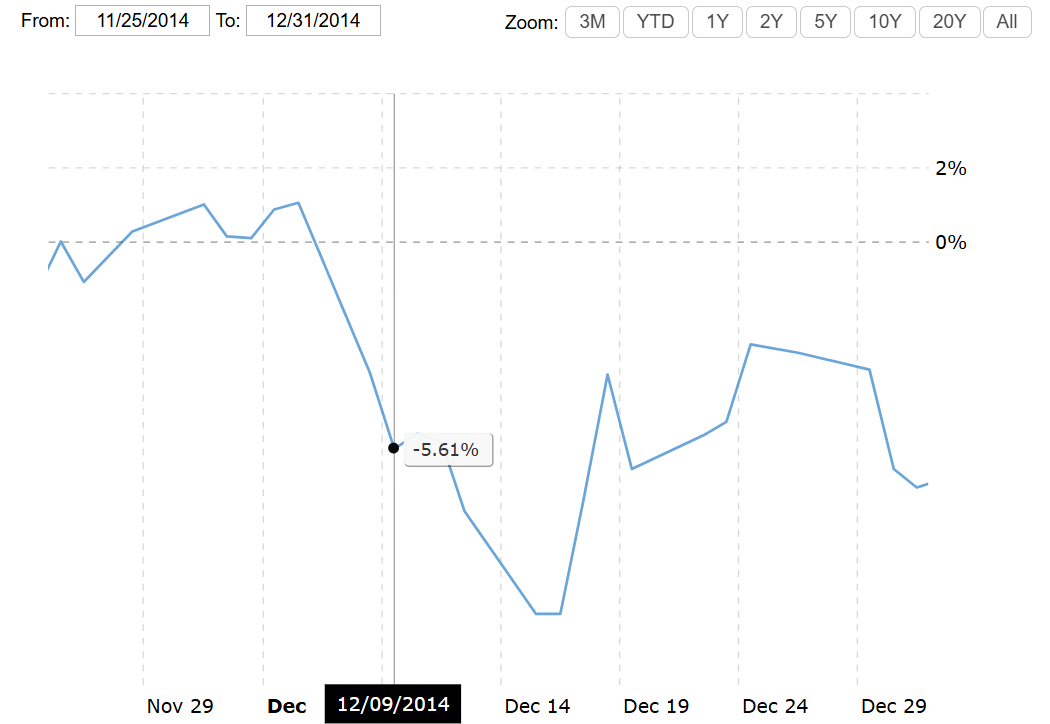
\includegraphics[width=10cm]{figures/sony_2014_short.png} 
\caption[Grafico Sony Pic short]{Impatto a breve termine Sony Picture hack}\label{fig:sPic1}
\end{center}
\end{figure}

Sul lungo periodo l'andamento si \`e probabilmente svincolato dalla discesa iniziale, anche  grazie alla diffusa gamma di attivit\`a in di cui si occupa il gruppo \ref{fig:sPic2}. L'impatto quindi non \`e quantificabile in maniera semplice, ma \`e ragionevole pensare che il danno di immagine si sia protratto a lungo.\\
\begin{figure}[H] 
\begin{center} 
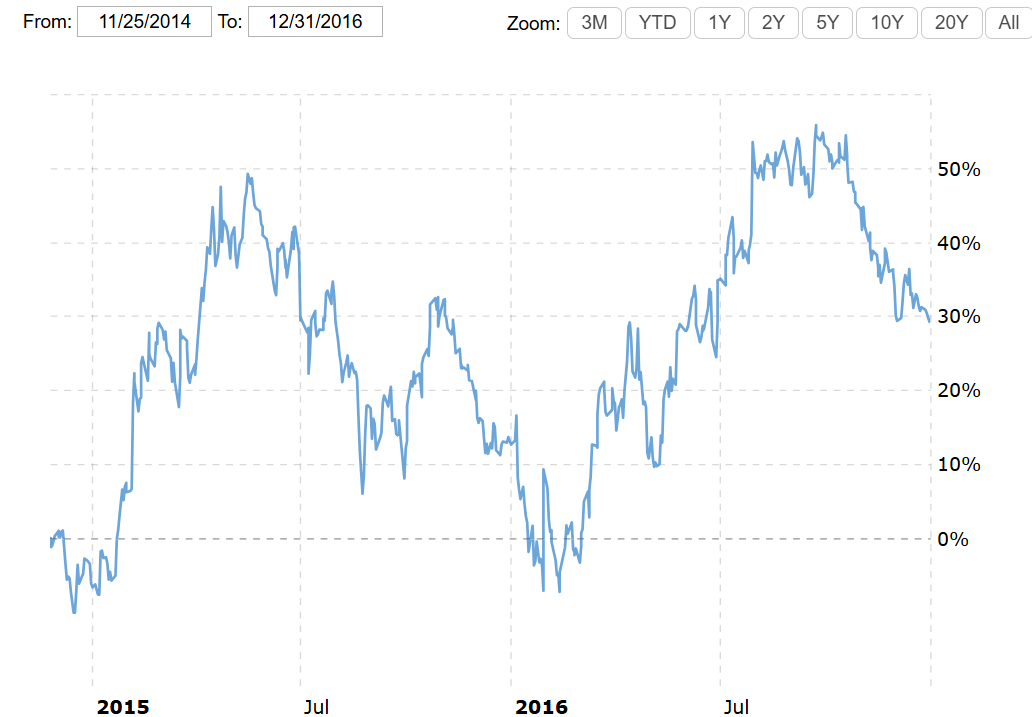
\includegraphics[width=10cm]{figures/sony_2014_long.png} 
\caption[Grafico Sony Pic long]{Impatto a lungo termine Sony Picture hack}\label{fig:sPic2}
\end{center}
\end{figure}
\subsection{Note}
La copertura dei media e la grande mole di notizie riguardanti il caso derivano dall'associazione dell'attacco alla Corea del Nord e ad un film in uscita, prodotto da SPE, ``The Interview'', in cui la storia sarebbe stata costruita attorno al tentato assassinio del leader Kim Jong Un.
Nella gestione della crisi, l'essere protagonisti di un evento tanto discusso ha sicuramente contribuito ad aggravare i danni d'immagine connessi alla vicenda\cite{SonyPic_buzzfeed}.\\

\section{Yahoo (2013, 2014)}
\subsection{Descrizione}
A settembre 2016 rende noto che nel 2014 sono stati rubati i dati personali di 500 milioni di utenti a seguito di un attacco di ingegneria sociale\cite{yahoo_book}.\\
Il 14 dicembre 2016 Yahoo comunica che, mentre investigava al riguardo, ha scoperto un secondo furto: durante agosto 2013 \`e avvenuto quello che ricordiamo come il pi\`u grande \textit{data breach} della storia. Inizialmente venne dichiarato si trattasse di 1 miliardo, poi, nel 2017 il dato si assester\`a solidamente sui 3 miliardi di account di cui sono state diffuse informazioni\cite{yahoo_book}\cite{yahoo_guardian}.
\subsection{Impatto diretto}
L'azienda era in fase di acquisizione da parte di Verizon che, ritrattando il prezzo a ribasso, pass\`o da un'offerta di \$4,83 miliardi ad un prezzo finale, nel 2017, di \$4,48 determinando una perdita effettiva di \$350 milioni\cite{yahoo_book}.\\
Inoltre i procedimenti portarono l'azienda a pagare altri \$35 milioni per un patteggiamento con la SEC e \$117 milioni per risarcire gli utenti colpiti.\\
\subsection{Impatto indiretto}
Nel breve termine possiamo osservare una discesa di quasi il 10\% da settembre alla fine di dicembre 2016 prima di una crescita che anticipa l'acquisizione.\\
\begin{figure}[H] 
\begin{center} 
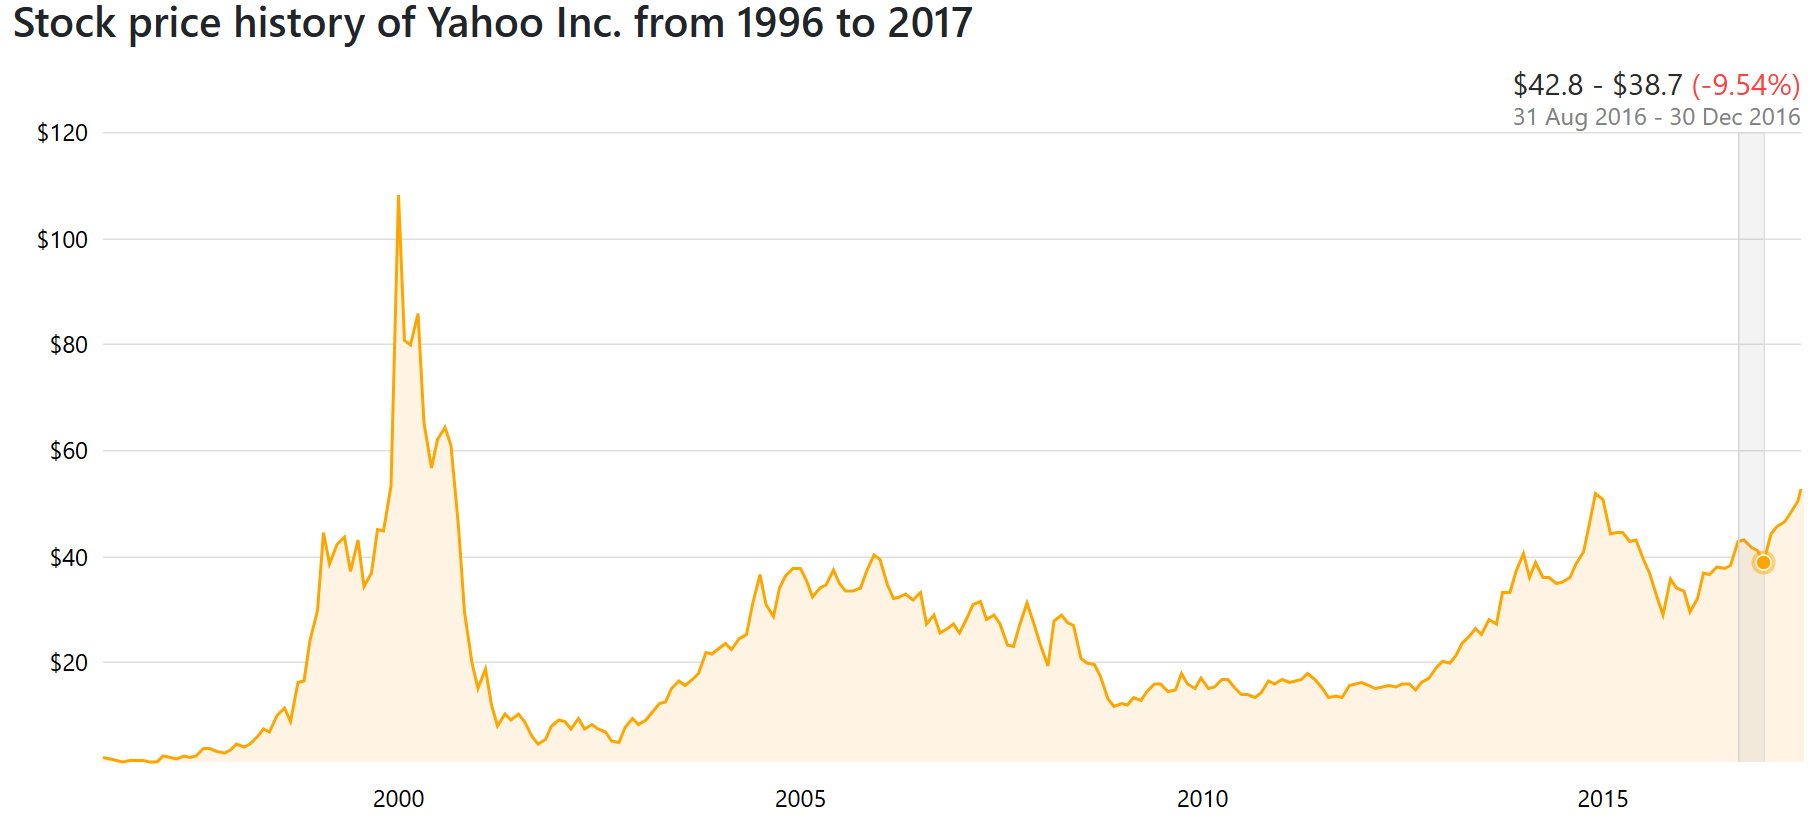
\includegraphics[width=10cm]{figures/yahoo_short.png} 
\caption[Grafico Yahoo short]{Impatto a breve termine Yahoo data breach}\label{fig:yahoo1}
\end{center}
\end{figure}

Nel periodo prossimo all'acquisto di Yahoo, Verizon subisce un calo del 6\%. Osservare oltre l'andamento rischia di essere fuorviante per via dei diversi componenti dell'azienda al tempo, ma le azioni seguono un trend in crescita\\
\begin{figure}[H] 
\begin{center} 
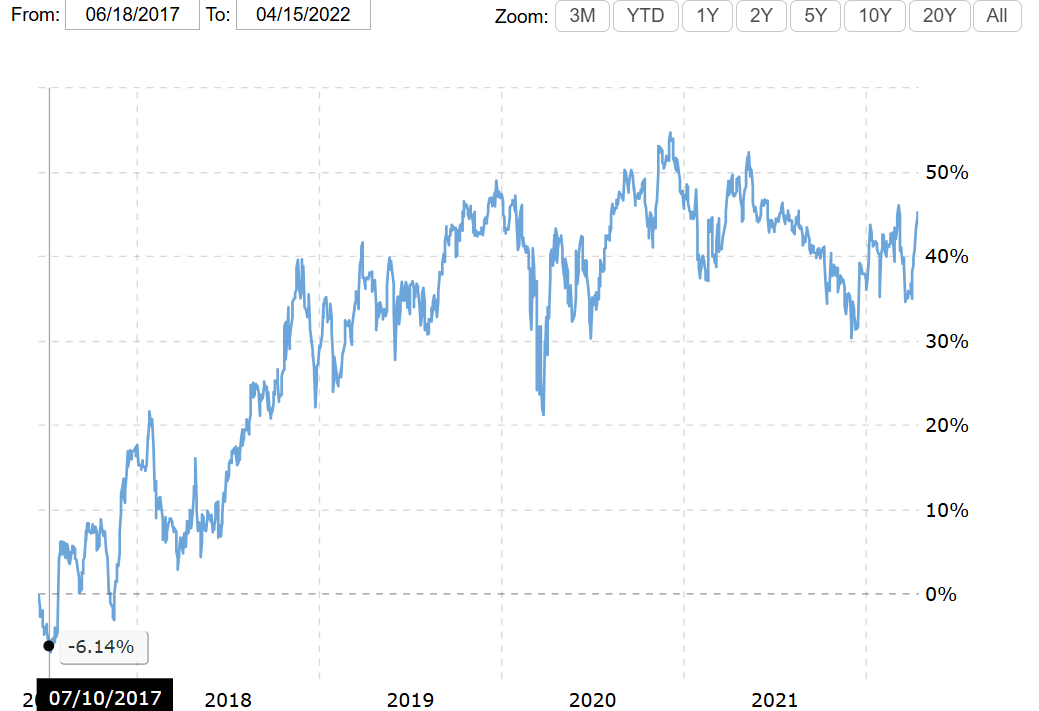
\includegraphics[width=10cm]{figures/yahoo-verizon-long.png} 
\caption[Grafico Verizon (Yahoo) long]{Impatto a lungo termine Verizon (Yahoo) data breach}\label{fig:yahoo2}
\end{center}
\end{figure}
\subsection{Note}
\begin{enumerate}
    \item la fonte dei grafici storici di yahoo \`e \href{https://companiesmarketcap.com/yahoo/stock-price-history}{https://companiesmarketcap.com/}, in quanto non \`e stato possibile procurarsi dati pi\`u precisi di una azienda il cui ticker non esiste pi\`u;
    \item la gestione delle comunicazioni da parte dell'azienda \`e stata tardiva a dir poco, contribuendo ad aggravarne la posizione nei confronti dell'opinione pubblica e della legge.
\end{enumerate}
\section{Uber (2016, 2022)}
\subsection{2016}
\subsubsection{Descrizione}
Il \textit{data breach} avvenne ad ottobre 2016, ma la divulgazione risale a ben un anno dopo, grazie ad un cambio di dirigenza. I rischi che ha corso nel gestire ambiguamente il caso hanno rischiato di avere conseguenze penali\cite{Uber_plusEquifaxAndYahoo}.\\ 
\subsubsection{Impatto diretto}
L'azienda, oltre al riscatto pagato agli hacker per eliminare i dati rubati, ha concordato coi 50 stati americani il pagamento di una multa di \$148 milioni.\\
\subsubsection{Impatto indiretto}
Al tempo l'azienda non era quotata, quindi non \`e possibile analizzare questo aspetto, se non osservando il caso del 2022.\\
\subsubsection{Note}
Una aggravante \`e stata sicuramente la gestione consapevolmente ingannevole. Rivel\`o per esempio  l'esistenza del \textit{breach} a SoftBank, permettendo poi che comprasse una buona parte della compagnia a prezzo ribassato\cite{Uber_plusEquifaxAndYahoo}.\\   
\subsection{2022}
\subsubsection{Descrizione}
Tramite ingegneria sociale l'attaccante \`e riuscito ad entrare nel sistema di condivisione di informazioni aziendali Slack, con conseguente arresto forzato di alcuni servizi da parte dell'azienda il 13 settembre 2022\cite{Uber_2022}.\\
\subsubsection{Impatto diretto}
La prontezza della reazione ha permesso di contenere le conseguenze dirette dell'attacco, evitando eventuali sanzioni.\\ 
\subsubsection{Impatto indiretto}
Il mercato ha invece reagito pi\`u bruscamente di quanto visto fin'ora \ref{fig:ubr1}, con un picco verso il basso di -10\% rispetto al giorno della scoperta (ancor pi\`u pronunciato se prendiamo in esame il 15 settembre, data della dichiarazione). Ad un mese di distanza la discesa rallenta ma non si arresta.\\

\begin{figure}[H] 
\begin{center} 
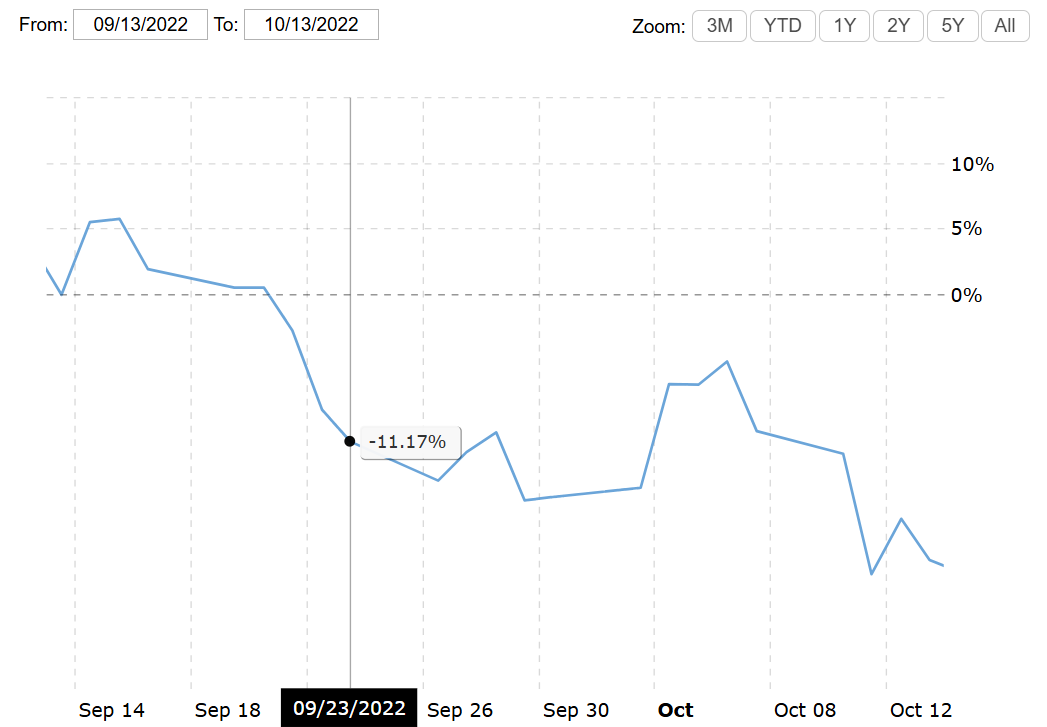
\includegraphics[width=10cm]{figures/uber_2022_short.png} 
\caption[Grafico Uber 2022 short]{Impatto a breve termine Uber 2022}\label{fig:ubr1}
\end{center}
\end{figure}

Per tornare in pari ci vogliono pi\`u di sette mesi, indice che i precedenti attacchi avevano lasciato un segno importante nella reputazione dell'azienda.\\

\begin{figure}[H] 
\begin{center} 
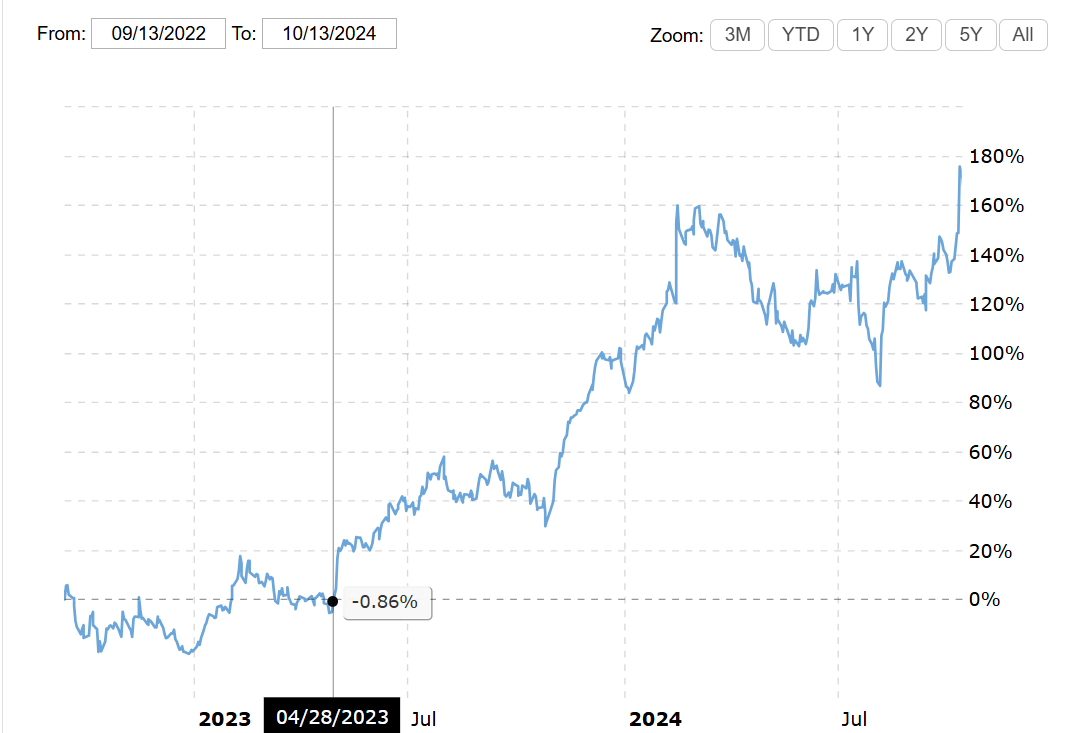
\includegraphics[width=10cm]{figures/uber_2022_long.png} 
\caption[Grafico Uber 2022 long]{Impatto a lungo termine Uber 2022}\label{fig:ubr2}
\end{center}
\end{figure}

\subsubsection{Note}
Il primo \textit{data breach} e le sue conseguenze sono servite a Uber per cambiare approccio alla sicurezza e migliorare diversi aspetti\cite{Uber_2022}.

\section{FedEx - NotPetya (2017)}
\subsection{Descrizione}
Il \textit{ransomware} NotPetya fu un attacco diffuso su larga scala, con epicentro in Ucraina, a giugno del 2017. Sua  peculiarit\`a era di non essere stato concepito per scopi di lucro, quanto pi\`u invece per causare disordine e distruzione\cite{FedEx_evolutionOfRansom}, secondo un rapporto della Casa Bianca i danni ammontarono complessivamente a \$10 miliardi\cite{FedEx_wired}.\\
In questo contesto, l'azienda FedEx Corporation, che aveva da poco fatto acquisizioni in Europa (TNT Express), affront\`o grossi disservizi nel vecchio continente che complicarono i processi di assimilazione\cite{FedEx_10K_report_2018}.\\
\subsection{Impatto diretto}
Nel bilancio depositato a SEC si stimano le perdite intorno ai \$400 milioni che rallentarono la crescita durante il primo quarto dell'anno fiscale (giugno-agosto 2017).\\
\subsection{Impatto indiretto}
Essendo l'azienda distribuita, e in forte crescita negli Stati Uniti, l'impatto distruttivo di NotPetya non \`e clamoroso quanto ci si aspetterebbe da uno dei pi\`u costosi attacchi della storia. Di fatti, dal 27 giugno 2017 (giorno dell'attacco) le azioni crescono ed iniziano una discesa solo qualche tempo dopo, scendendo fino a -5\%.\\
\begin{figure}[H] 
\begin{center} 
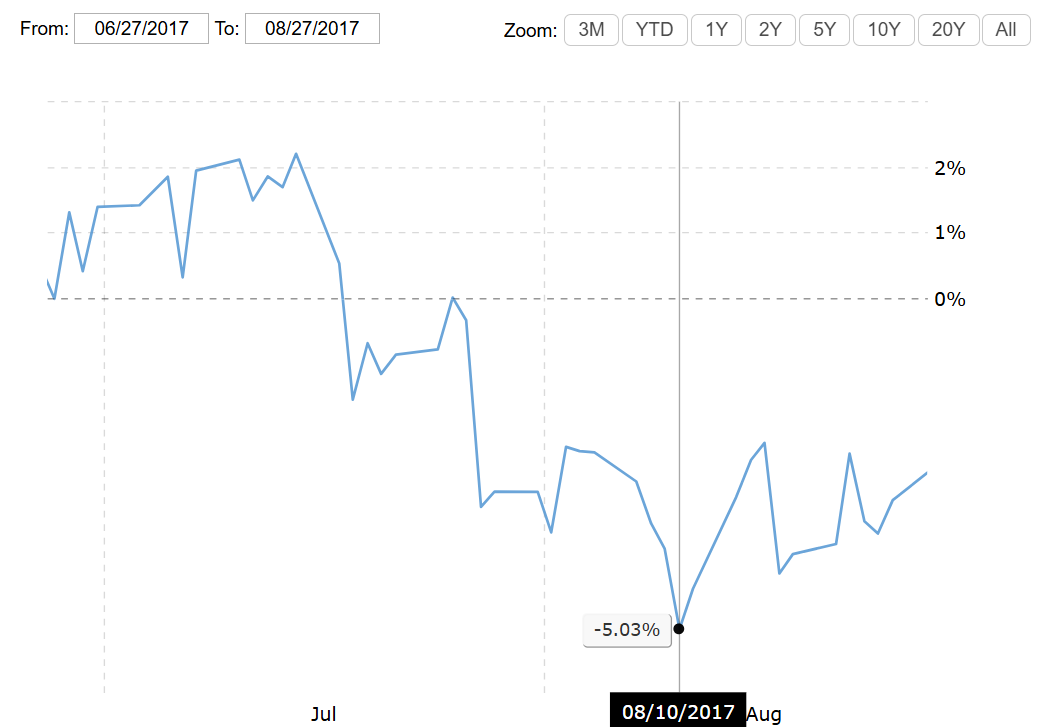
\includegraphics[width=10cm]{figures/fedex_short.png} 
\caption[Grafico FedEx NotPetya short]{Impatto a breve termine NotPetya su FedEx}\label{fig:fdx1}
\end{center}
\end{figure}

Come gi\`a discusso ci sono segnali di una ripresa abbastanza forte, che in mancanza dell'attacco, sarebbero potuti essere lo specchio di una crescita  ancora pi\`u importante.

\begin{figure}[H] 
\begin{center} 
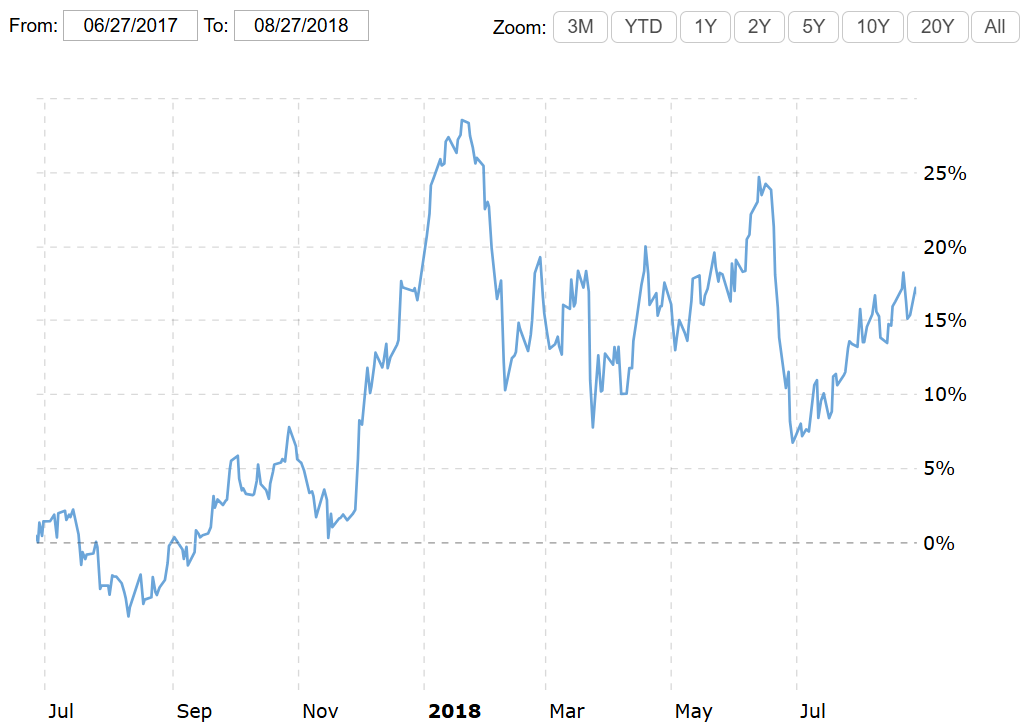
\includegraphics[width=10cm]{figures/fedex_long.png} 
\caption[Grafico FedEx NotPetya long]{Impatto a lungo termine NotPetya su FedEx}\label{fig:fdx2}
\end{center}
\end{figure}

\subsection{Note}

La diffusione cos\`i ampia di un attacco lo assimila, agli occhi dell'opinione pubblica, ad un disastro naturale o comunque ad un fattore esterno, intaccando pi\`u tramite costi diretti che indiretti le aziende coinvolte. I danni di immagine risultano quindi significativamente contenuti.

\section{Equifax (2017)}
\subsection{Descrizione}
L'8 settembre 2017, l'agenzia di informazioni creditizie al consumo americana Equifax rilascia un comunicato in cui dichiara che ha subito un \textit{data breach} che interessa  148 milioni di cittadini statunitensi. L'attacco \`e stato possibile grazie al mancato aggiornamento tempestivo di alcuni server con una specifica vulnerabilit\`a nota, presente dell'URL\cite{Equifax_case_study_2}.\\
\subsection{Impatto diretto}
Come conseguenza della grande quantit\`a di cause indette contro Equifax, l'azienda arriv\`o a concordare un impegno monetario di \$575-\$700 milioni\cite{Equifax_settlement}.\\
\subsection{Impatto indiretto}
L'impatto fu molto pesante, a distanza di tre giorni osserviamo un calo dell' 8,20\%, che va oltre il 20\% a met\`a settembre. Questo \`e dovuto ad una massiccia vendita delle azioni, pari a \$1,8 milioni\cite{Uber_plusEquifaxAndYahoo}\\

\begin{figure}[H] 
\begin{center} 
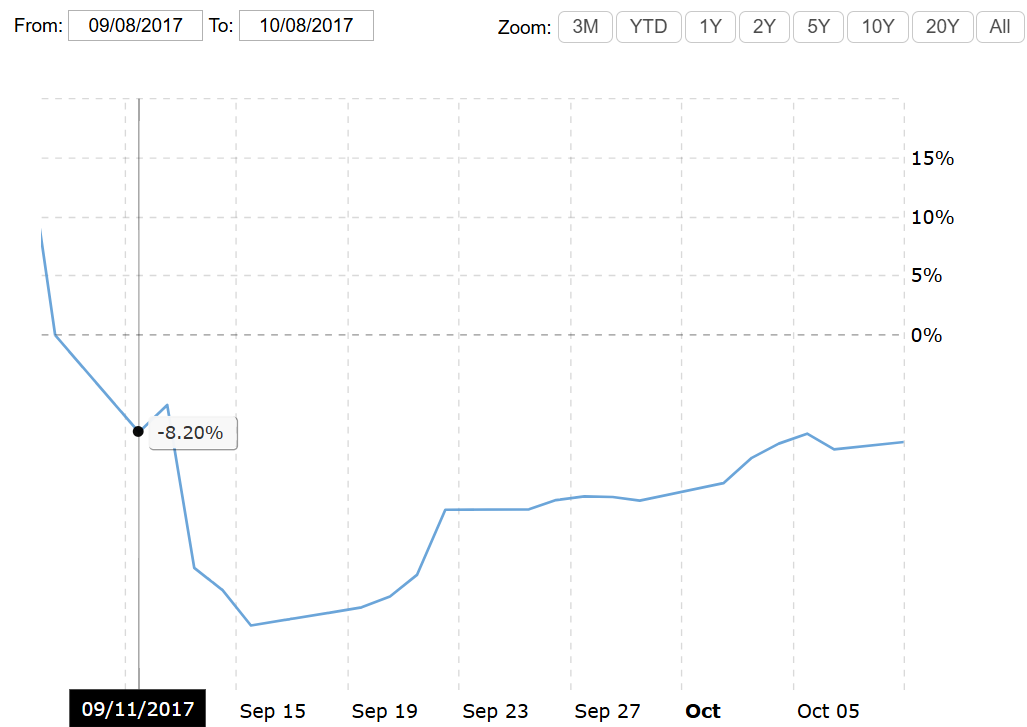
\includegraphics[width=10cm]{figures/equifax_short.png} 
\caption[Grafico Equifax short]{Impatto a breve termine Equifax breach}\label{fig:eqx1}
\end{center}
\end{figure}

Sul lungo periodo l'azienda fatica a risollevarsi, complici le pesanti sanzioni e la perdita di fiducia degli investitori.\\

\begin{figure}[H] 
\begin{center} 
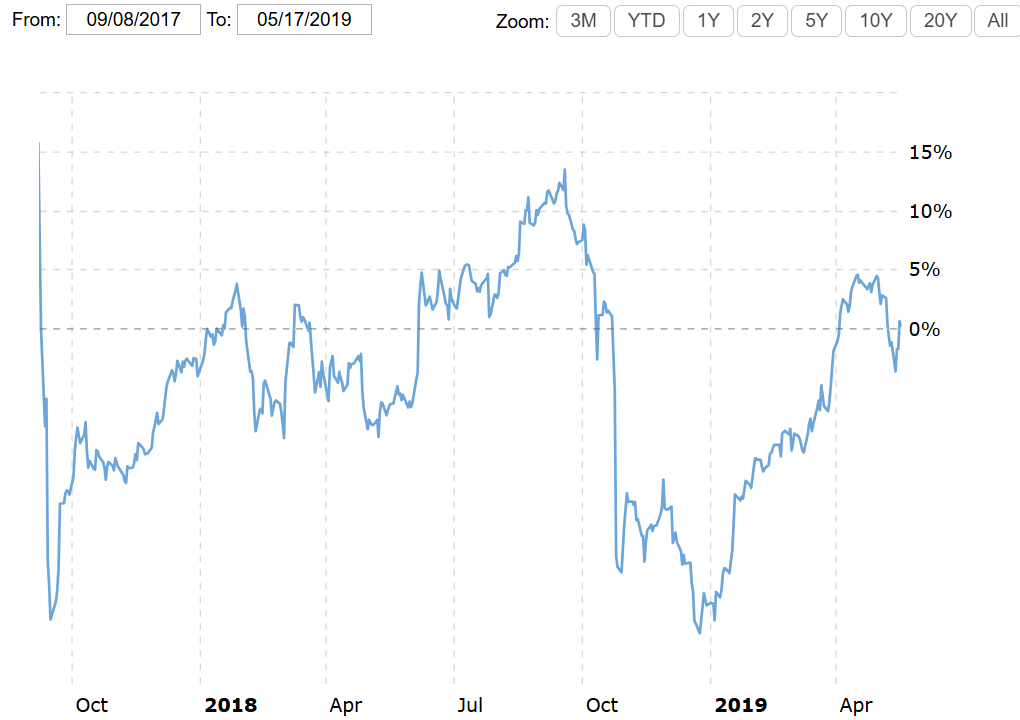
\includegraphics[width=10cm]{figures/equifax_long.png} 
\caption[Grafico Equifax long]{Impatto a lungo termine Equifax breach}\label{fig:eqx2}
\end{center}
\end{figure}

\subsection{Note}
Pare che il fatto che il \textit{breach} fosse noto alla dirigenza gi\`a da inizio agosto 2017\cite{Uber_plusEquifaxAndYahoo} sia stata, insieme al tipo di informazioni perse, una pesante aggravante in ambito legale.\\
\section{British Airways (2018)}
\subsection{Descrizione}
Il \textit{data breach}, attuato tramite l'iniezione di 22 linee di codice Javascript malevolo via URL (\textit{cross site scripting}, XSS), che colp\`i la compagnia aerea del Regno Unito, British Airways, venne reso pubblico il 6 settembre 2018 da un comunicato pubblico del \textit{National CyberSecurity Centre}. Le vittime, le cui stime iniziali ne dichiaravano $380\,000$, si scoprono ad ottobre essere ben $565\,000$, di cui sono trapelati nomi, email e informazioni delle carte di credito.\cite{BritAir} 
\subsection{Impatto diretto}
L'azienda ha sostenuto una multa di \$20 milioni come conseguenza dell'attacco. \cite{BritAir} La pena ridotta \`e probabilmente una concessione dovuta alla successiva crisi causata dal COVID-19.\\
\subsection{Impatto indiretto}
La compagnia \`e nel gruppo \textit{International Airlines Group} e quotata nelle borse inglesi e spagnole, pertanto discuteremo l'andamento di quest'ultimo tramite i dati ufficiali di \href{https://www.londonstockexchange.com/stock/}{\textit{London Stock Exchange}}.\\
Il gruppo, come evidenziato nelle fonti\cite{BritAir} ha una perdita quasi immediata del 2\%, e continua a scendere durante tutto il mese successivo.

\begin{figure}[H] 
\begin{center} 
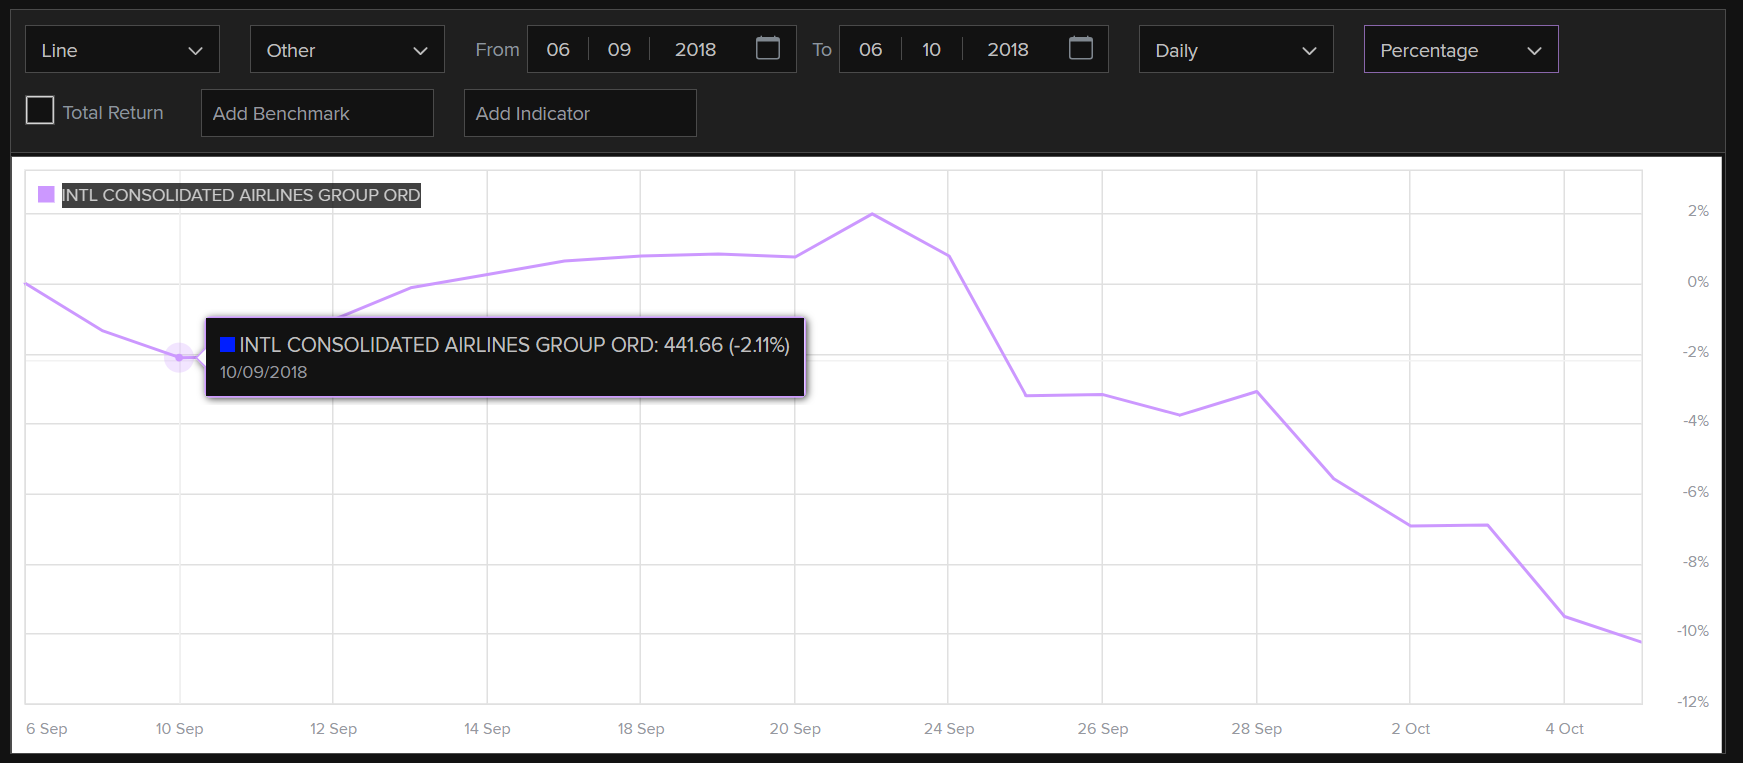
\includegraphics[width=10cm]{figures/britAir_short.png} 
\caption[Grafico British Airways short]{Impatto a breve termine British Airways}\label{fig:britair1}
\end{center}
\end{figure}

Nel lungo periodo le azioni risentono del danno di immagine fino all'inizio del 2020, in cui per\`o, la compagnia ha ricadute legate all'inizio della pandemia del COVID-19.\\

\begin{figure}[H] 
\begin{center} 
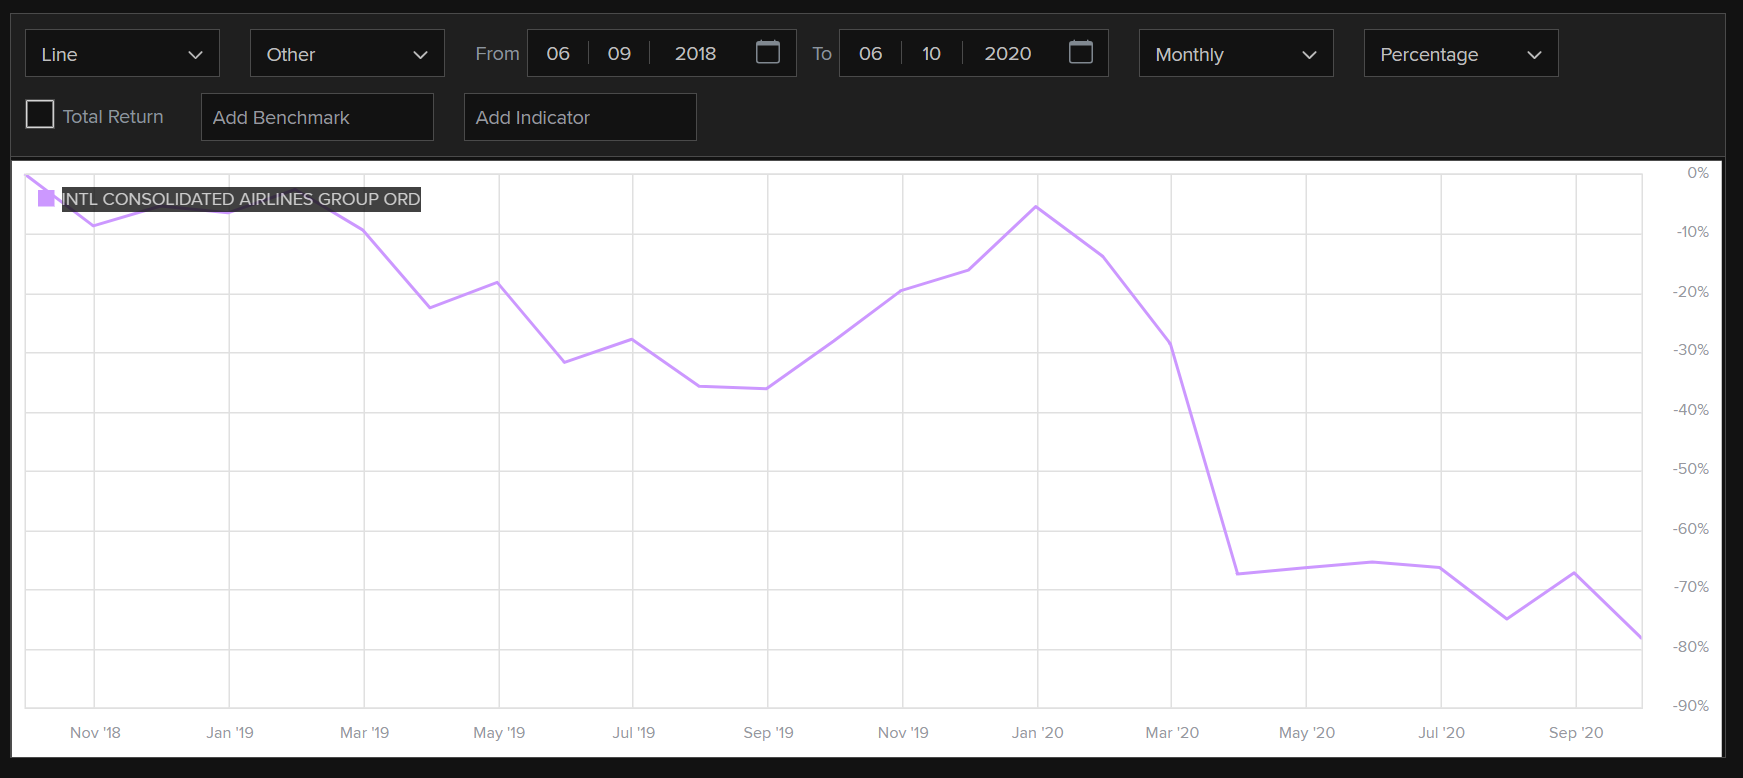
\includegraphics[width=10cm]{figures/britAir_long.png} 
\caption[Grafico British Airways long]{Impatto a lungo termine  British Airways}\label{fig:britair2}
\end{center}
\end{figure}

\section{Marriot International (2018)}
\subsection{Descrizione}
L'attacco si distribuisce su un ampio lasso di tempo: nel 2014, tramite accesso fisico ad un terminale con permessi di amministratore, viene installato un \textit{malware} nella rete di Starwood, agenzia alberghiera statunitense. Dopo aver trovato la chiave di decrittazione dei database e aver esfiltrato i dati, gli attaccanti cifrarono nuovamente le informazioni per non lasciare tracce. Rimasero tali anche dopo l'acquisizione di Starwood da parte di Marriott International nel 2016, tanto che l'attacco pass\`o  inosservato fino all'8 settembre 2018. Seguirono investigazioni che culminarono nella dichiarazione del 30 novembre 2018, in cui si rivelava la diffusione di informazioni di approssimativamente 500 milioni di clienti in tutto il mondo\cite{Marriott_ResGate}\cite{Marriott_customer_perception}.\\ 
\subsection{Impatto diretto}
Come spese di riparazione interne Marriott dichiara \$30 milioni \cite{Marriott_ResGate}, in aggiunta pag\`o anche una multa di \textsterling18,4 milioni al Regno Unito \cite{Marriott_actual_fine}, sebbene  inizialmente le cifre dichiarate fossero intorno ai \textsterling99 milioni.\\ 
\subsection{Impatto indiretto}
Il giorno dell'annuncio registra un calo di pi\`u del 5\% arrivando oltre  -17\% sotto Natale. Marriott dichiar\`o una perdita stimata di \$1 miliardo dovuta alla perdita di fiducia dei clienti\cite{Marriott_ResGate}.\\

\begin{figure}[H] 
\begin{center} 
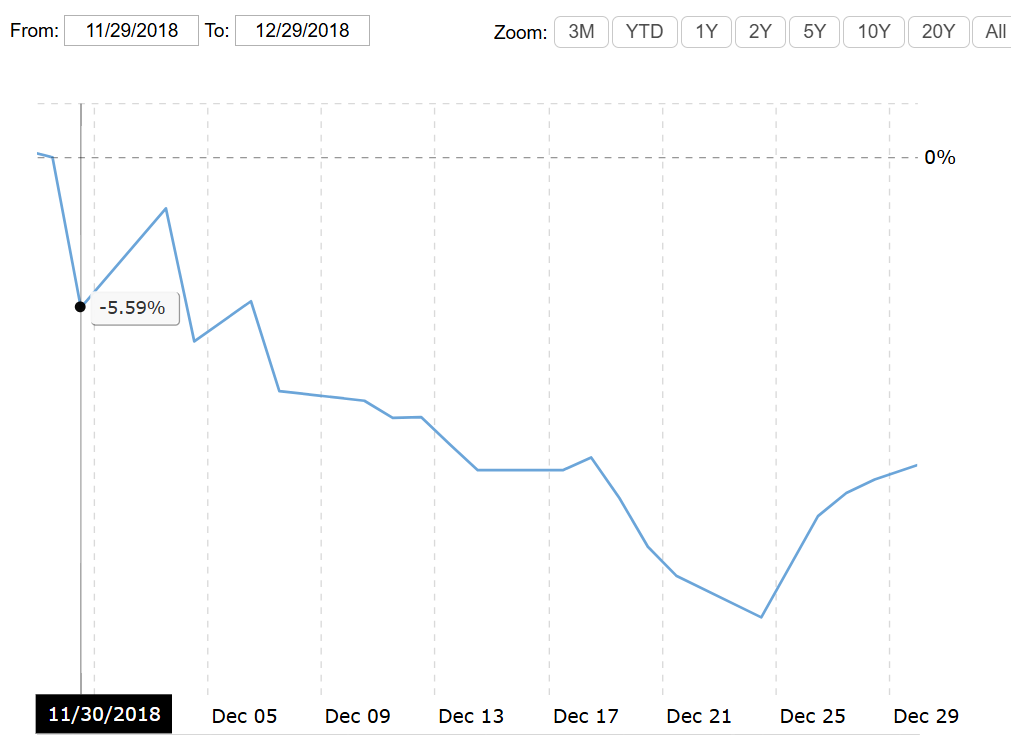
\includegraphics[width=10cm]{figures/marriott_short.png} 
\caption[Grafico Marriott short]{Impatto a breve termine Marriott International data breach}\label{fig:mrt1}
\end{center}
\end{figure}

Negli anni successivi torna a crescere fino ad inizio 2020, anche qui, si suppone dovuta alla contrazione del mercato di quel periodo.\\

\begin{figure}[H] 
\begin{center} 
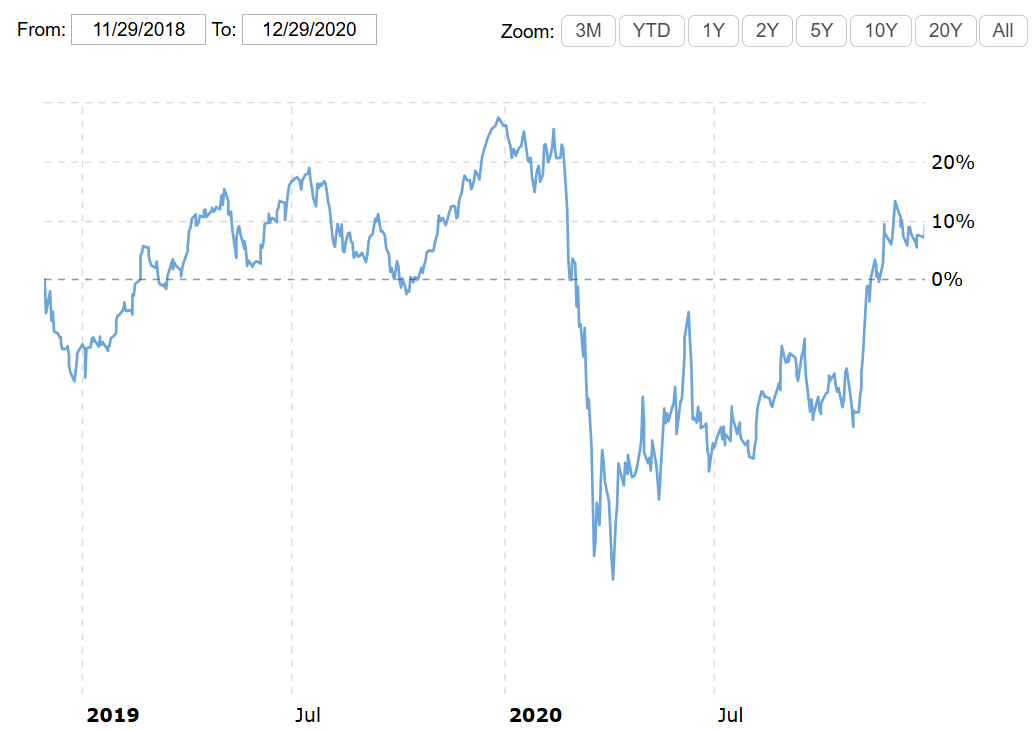
\includegraphics[width=10cm]{figures/marriott_long.png} 
\caption[Grafico Marriott long]{Impatto a lungo termine  Marriott International data breach}\label{fig:mrt2}
\end{center}
\end{figure}

\subsection{Note}
La crisi \`e stata generata da errori nel controllo dei sistemi informativi e della rete della societ\`a acquisita, evidenziando come l'espansione di un'azienda in tal modo sia fonte di vulnerabilit\`a talvolta inaspettate. Per quanto quest'ultima abbia provato a scaricare la responsabilit\`a dell'accaduto altrove, risulta evidente quanto sia in realt\`a un compito cruciale da svolgere durante grandi o piccole operazioni di fusione.\\ 
\section{Capital One (2019)}
\subsection{Descrizione}
La holding bancaria Capital One Financial Corporation scopre, tramite una mail proveniente da un esterno di un \textit{data breach} che ha interessato 100 milioni di cittadini statunitensi e 6 milioni canadesi, pubblicher\`a quindi un comunicato al riguardo il 29 luglio 2019\cite{CapitalOne_case_study}.
\subsection{Impatto diretto}
Oltre alla multa di \$80  milioni, ha poi raggiunto un accordo di risarcimento dal valore di \$190 milioni ad inizio 2022 \cite{CapitalOne_settlement}.
\subsection{Impatto indiretto}
Come \`e osservabile in figura \ref{fig:cpto1}, al giorno del comunicato \`e seguito un crollo di quasi il 6\% e le azioni hanno continuato la discesa per tutto il mese successivo.\\ 
\begin{figure}[H] 
\begin{center} 
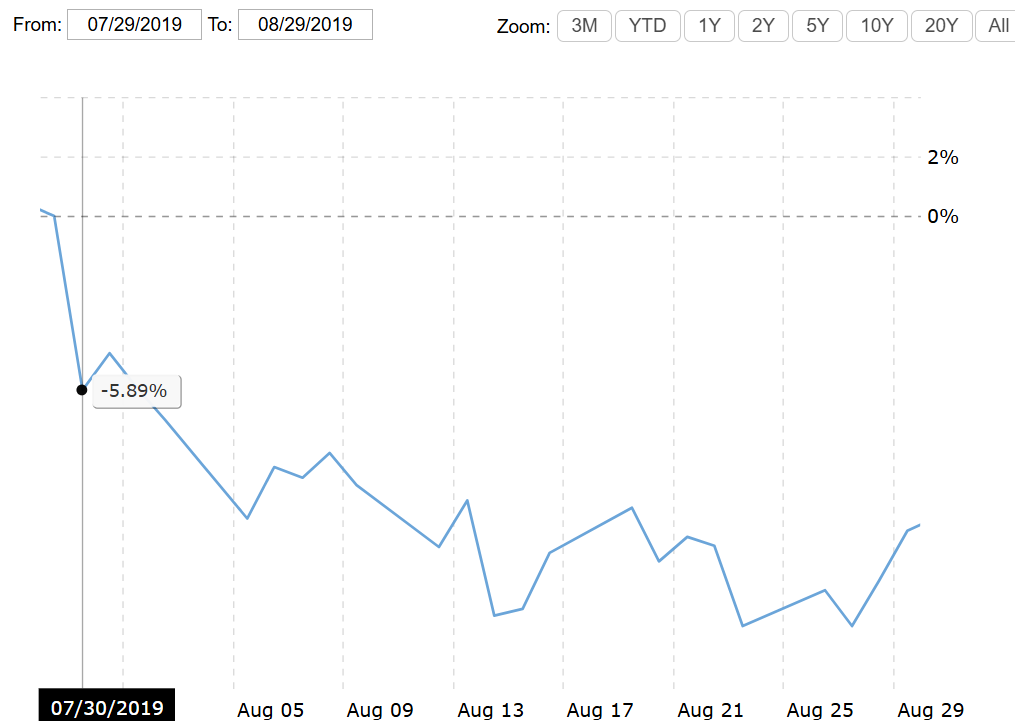
\includegraphics[width=10cm]{figures/capitalOne_short.png} 
\caption[Grafico Capital One short]{Impatto a breve termine Capital One}\label{fig:cpto1}
\end{center}
\end{figure}

Ormai \`e evidente il trend di ripresa (in questo caso moderata) e crollo ad inizio 2020, qui presente anche se la holding non \`e direttamente connessa a settori turistici, a evidenziare la pervasivit\`a della crisi finanziaria seguita al Covid-19.\\

\begin{figure}[H] 
\begin{center} 
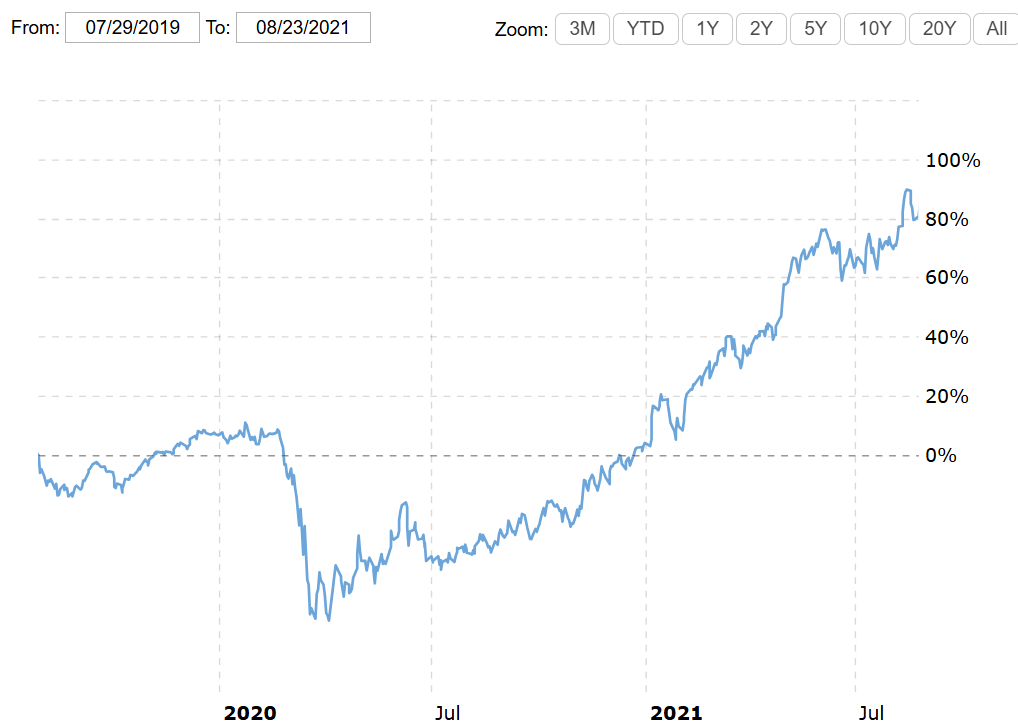
\includegraphics[width=10cm]{figures/CapitalOne_long.png} 
\caption[Grafico Capital One long]{Impatto a lungo termine  Capital One}\label{fig:cpto2}
\end{center}
\end{figure}
\subsection{Note}
Anche se molte fonti non individuano in Capital One errori grossolani, il percepito e la risposta del mercato sono stati netti.\\
\section{SolarWinds (2020)}
\subsection{Descrizione}
L'azienda di sviluppo di software aziendale SolarWinds \`e stata coinvolta, nel corso del 2020, in un \textit{supply chain attack} che l'ha vista protagonista della distribuzione di \textit{malware}.\\
A febbraio 2020, dopo aver ottenuto l'accesso alla rete aziendale, viene iniettato codice malevolo all'interno del prodotto Orion contenente una \textit{backdoor}, questi, che avrebbe poi assunto il nome di SUNBURST, venne distribuito in un aggiornamento software a partire da marzo, sfruttando i certificati che garantivano l'autenticit\`a della sorgente per rimanere occultato. Seguirono attacchi mirati fino all'8 dicembre 2020, in cui l'agenzia di cybersicurezza FireEye non si accorse del furto di alcuni suoi strumenti, portando poi alla rivelazione al pubblico in data 13 dicembre 2020.\\
L'attacco colp\`i tra i $17\,000$ e i $18\,000$ clienti di SolarWinds, compresi enti governativi \cite{SolarWinds_lessons}\cite{SolarWinds_analysis}\cite{SolarWinds_conference}.\\

\subsection{Impatto diretto}
Stime riportano il costo per le compagnie assicurative di \$90 milioni. SolarWinds in particolare ha poi concordato con la SEC una sanzione di \$26 milioni \cite{SolarWinds_2022_SEC}. 
\subsection{Impatto indiretto}
Possiamo vedere la portata distruttiva che ha avuto l'attacco sulle azioni, con una discesa pari a -34,66\% in un solo mese, e l'inizio di un trend discendente che \`e durato pi\`u di un anno.\\
\begin{figure}[H] 
\begin{center} 
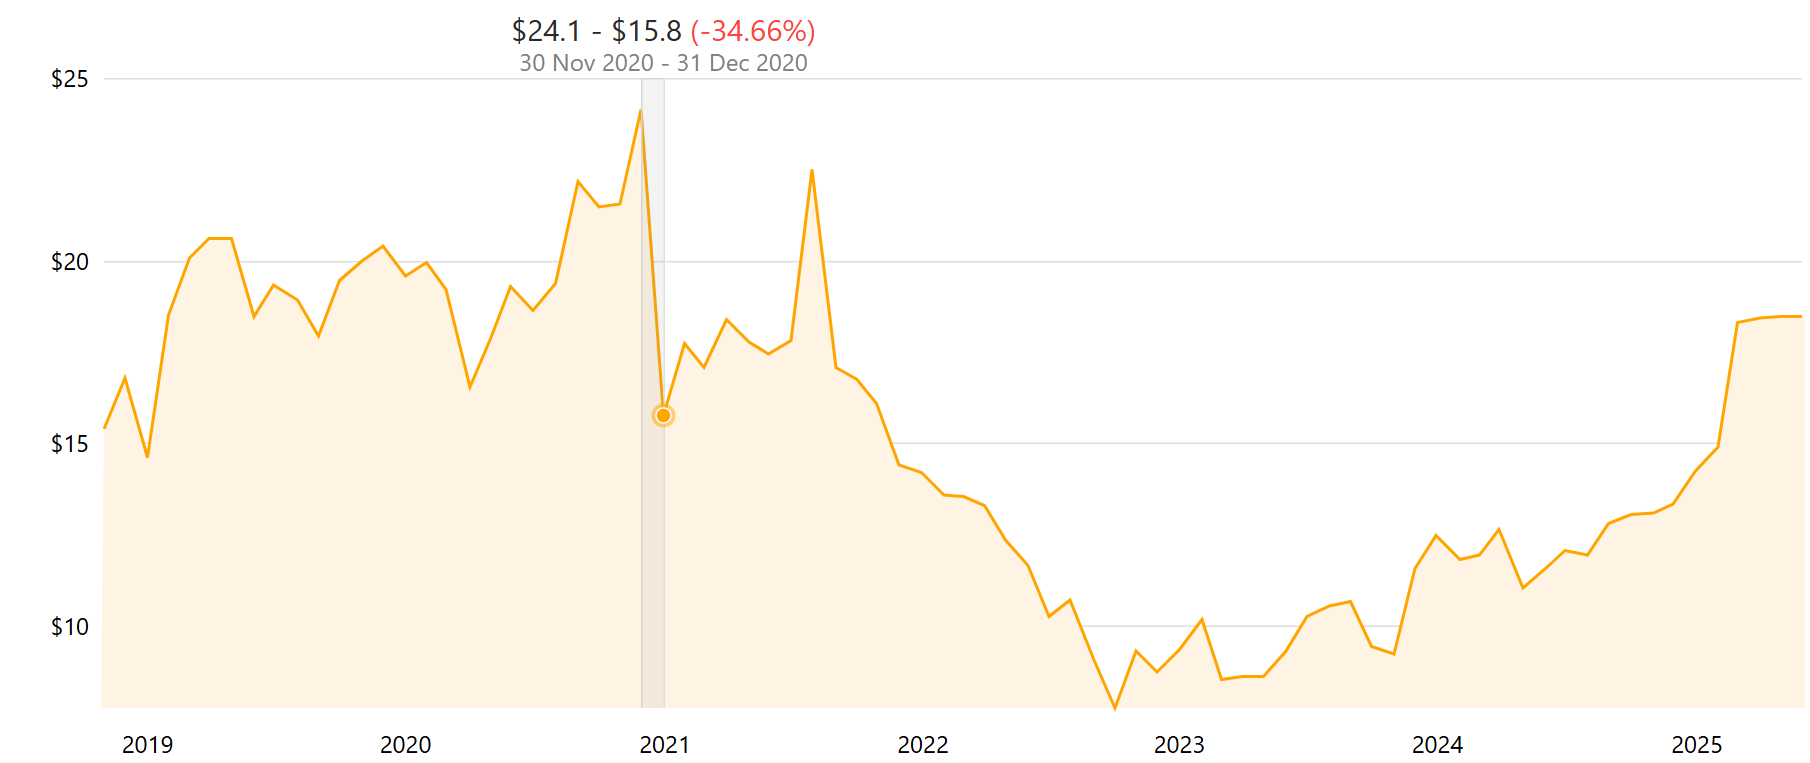
\includegraphics[width=10cm]{figures/solarwinds.png} 
\caption[Grafico SolarWinds]{Impatto SolarWinds supply chain attack}\label{fig:slrw}
\end{center}
\end{figure}
\subsection{Note}
La compagnia \`e stata acquistata nella pima met\`a del 2025, perci\`o i dati provengono nuovamente da \href{https://companiesmarketcap.com/solarwinds/stock-price-history}{https://companiesmarketcap.com/}\\

\section{Colonial Pipeline (2021)}
\subsection{Descrizione}
L'attacco \textit{ransomware} alla compagnia di trasporto di carburanti \`e stato compiuto tramite BEC (tipo particolare di ingegneria sociale) con lo scopo di ottenere un riscatto di \$4,4 milioni in BitCoin.\\
Ricevuta la richiesta di riscatto, il 7 maggio 2021, la dirigenza di Colonial Pipeline decise di arrestare l'imipianto e pagare gli attaccanti nel tentativo li limitare i danni \cite{ColonialPipe_IEEE}.
\subsection{Impatto diretto}
Il riscatto, sebbene sia stata recuperata una parte (\$2,3 milioni) rimane un costo affrontato dall'azienda \cite{ColonialPipe_IEEE}.\\
\subsection{Impatto indiretto}
Nonostante l'azienda non ha subito riduzioni di prezzo delle azioni, non essendo quotata, la comunit\`a ha sofferto la mancanza improvvisa del servizio, con aumenti esponenziali di prezzo e reazioni di panico generale \cite{ColonialPipe_context}.\\


\section{MGM Resorts (2023)}
\subsection{Descrizione}
Dal 10 settembre 2023 iniziano a trapelare indiscrezioni rigiuardo a comunicazioni tra l'FBI, il \textit{Nevada Gaming Control Board} e l'azienda multinazionale di intrattenimento, gioco d'azzardo e ospitalit\`a MGM Resorts, a seguito di cui, l'11 settembre, verr\`a rilasciato un comunicato in cui si annuncia l'arresto di alcuni servizi e l'inizio di indagini in merito ad un attacco informatico.\\
La natura del \textit{ransomware attack} diviene presto nota grazie alla rivendicazione da parte del gruppo di hacker ALPHV/BlackCat, che si \`e intrusa nel sistema tramite ingegneria sociale via telefonica (\textit{vishing}).\\
Nonostante la risposta pronta e la collaborazione stretta con le autorit\`a, sono state rubate informazioni riguardanti clienti e dipendenti, compromettendo la posizione di MGM Resorts International di fronte alla legge in materia di protezione dei dati personali \cite{MGMResorts_cybnews}.\\
\subsection{Impatto diretto}
MGM Resorts dichiara meno di \$10 milioni in spese di consulenza legale, coperti in larga parte da assicurazione \cite{MGM_8k_2023}. Ha in corso alcuni procedimenti , e ha patteggiato per un fondo di risarcimento per il caso del 2023 e uno precedente, del 2019, di \$45 milioni \cite{mgm_settlement}.  
\subsection{Impatto indiretto}
Nel rapporto straordinario a SEC si stima una perdita di  \$100 milioni nell'Adjusted Property EBITDAR (indicatore del fatturato ante tasse, interessi,  ammortamenti, deprezzamenti e spese di affitto aggiustato per escludere spese straordinarie).\\
Come si nota in figura \ref{fig:mgm1}, rispetto alle performances pre annuncio del \textit{data breach} e l'arresto dei servizi, viene registrato un calo superiore al 5\%, che tocca un picco di -20\% a inizio ottobre.\\
\begin{figure}[H] 
\begin{center} 
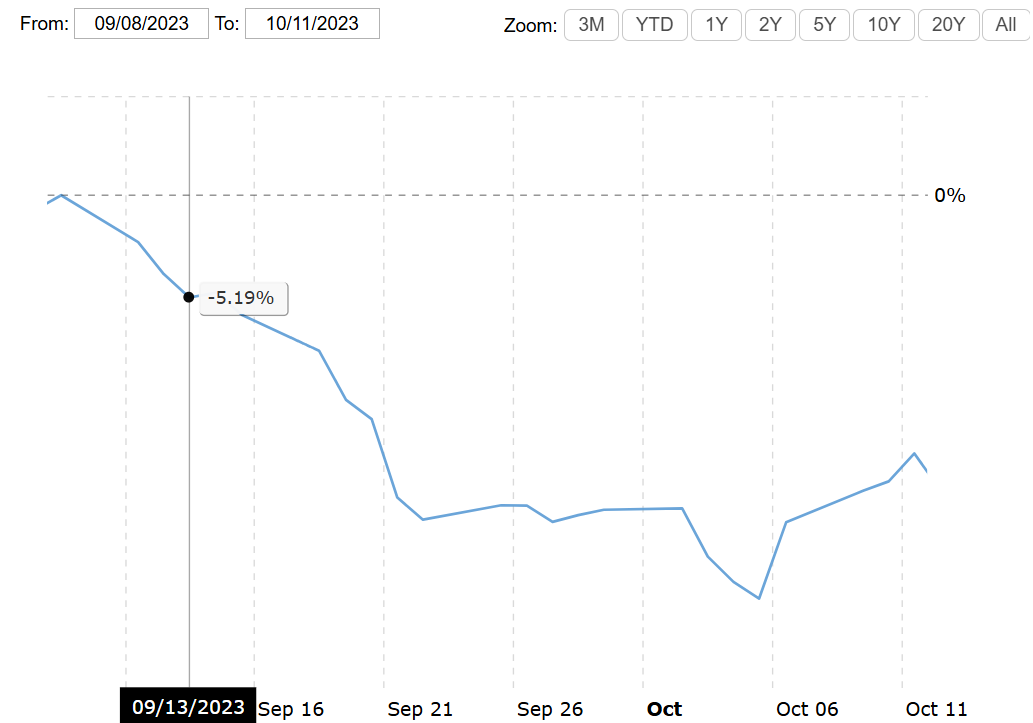
\includegraphics[width=10cm]{figures/MGM_short.png} 
\caption[Grafico MGM Resorts short]{Impatto a breve termine MGM Resorts}\label{fig:mgm1}
\end{center}
\end{figure}

Come da rapporto, era prevista una ripresa grazie ad un evento di Formula 1 \cite{MGM_8k_2023}, ma il calo successivo pu\`o essere connesso al danno di immagine subito.\\

\begin{figure}[H] 
\begin{center} 
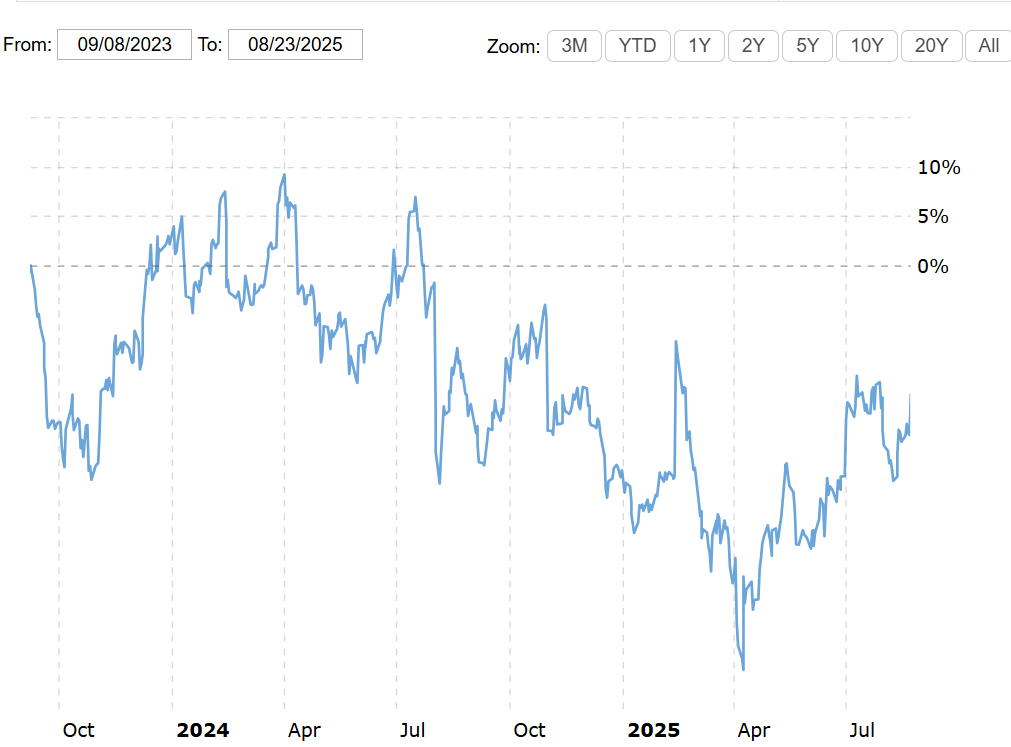
\includegraphics[width=10cm]{figures/MGM_long.png} 
\caption[Grafico MGM Resorts long]{Impatto a lungo termine  MGM Resorts}\label{fig:mgm2}
\end{center}
\end{figure}
\subsection{Note}
L'attacco \`e ben documentato anche grazie ad un rapporto pubblicato dagli attaccanti stessi che, per alcuni, pare vogliano cos\`i presentarsi come una controparte ragionevole nelle trattative che si sviluppano attorno ai loro attacchi \textit{ransomware}.\\
\section{Change Healthcare (2024)}
\subsection{Descrizione}
Change Healthcare Inc. \`e un gestore di pagamenti nel circuito sanitario statunitense parte della holding United Healthcare Group. Il 21 febbraio 2024 denuncia l'ingresso non autorizzato nei suoi sistemi da parte del, gi\`a menzionato, gruppo di hacker \textit{ransomware}  BlackCat. Per limitare i danni ha istantaneamente disattivato tutti i servizi, creando uno scompenso nel sistema sanitario nazionale. Nonostante tutto \`e stato stimato che siano trapelate le informazioni di 192,7 milioni di persone \cite{ChHealth_hipaa} \cite{ChHealth_lessons}.\\
\subsection{Impatto diretto}
Nel tentativo di recuperare i dati rubati, Change Healthcare, ha pagato \$22 milioni,a questo punto per\`o, il gruppo BlackCat si ritir\`o dalle trattative con il riscatto, e l'intermediario che le aveva gestite, ancora in possesso dei dati, ne chiese un secondo, che non fu corrisposto \cite{ChHealth_hipaa}. 
A questo si aggiungeranno le spese legali dei processi in corso. \\
Come impatti diretti, in un report sul terzo quarto dell'anno fiscale 2024, viene stimato a \$1,521 miliardi il costo diretto per United Health.\\
\subsection{Impatto indiretto}
Essenndo UH un gruppo ampio, e che le ripercussioni dell'attacco sono arrivate prima ad aziende pi\`u piccole, con limitata capacit\`a di gestire la crisi, \`e quindi ragionevole che il grafico non riporti una discesa istantanea, ma un picco verso il basso che parte quasi una settimana dopo l'annuncio del \textit{breach}.\\
La perdita nel breve termine si assesta comunque tra il 10\% e il 5\%.\\
\begin{figure}[H] 
\begin{center} 
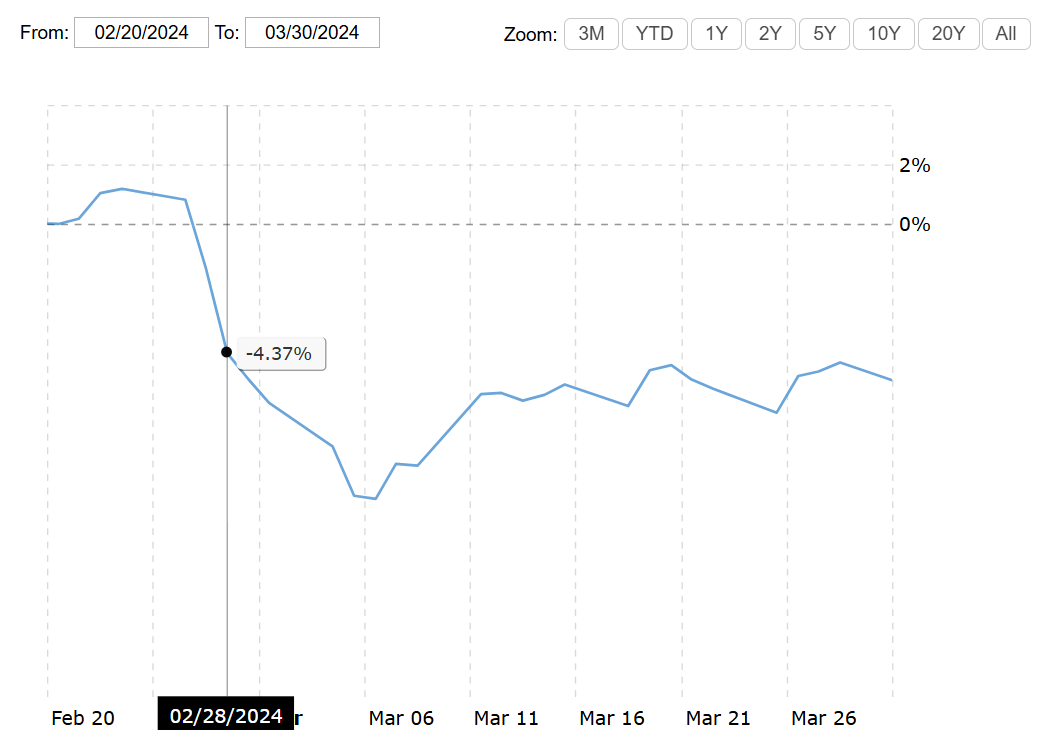
\includegraphics[width=10cm]{figures/chHealth_short.png} 
\caption[Grafico Change Healthcare short]{Impatto a breve termine Change Healthcare}\label{fig:chh1}
\end{center}
\end{figure}

Dopo luglio 2024 l'azienda ha iniziato il recupero, ma ad oggi pare in una crisi ancora peggiore di cui le sanzioni in arrivo, le perdite, gli ingenti prestiti fatti (\$9,7 miliardi \cite{ChHealth_lessons}) e il danno di immagine non sono protagonisti, ma hanno sicuramente un ruolo.\\

\begin{figure}[H] 
\begin{center} 
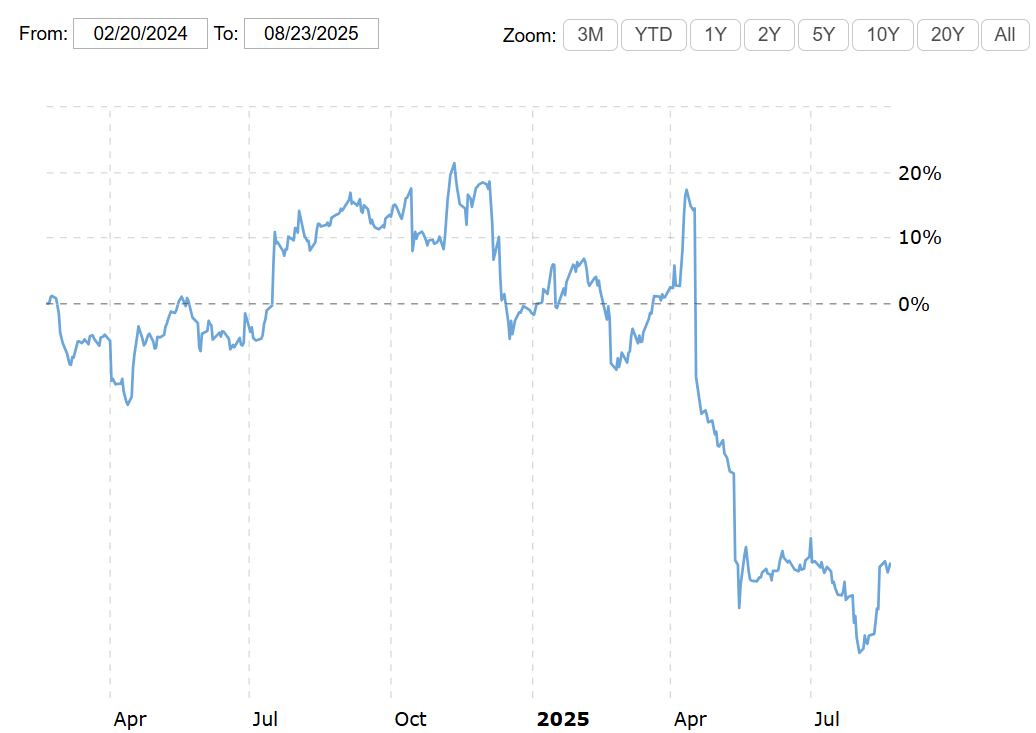
\includegraphics[width=10cm]{figures/chHealth_long.png} 
\caption[Grafico Change Healthcare long]{Impatto a lungo termine  Change Healthcare}\label{fig:chh2}
\end{center}
\end{figure}

\clearpage{\pagestyle{empty}\cleardoublepage}



%%%%%%%%%%%%%%%%%%%%%%%%%%%%%%%%%%%%%%%%
% Analisi dettagliata del precedente capitolo 
\chapter{Analisi dei dati aggregati}\label{chap:analisys}

Raccolgo in una tabella le analisi che si possono fare riguardo ai casi presentati, usando l'EBITDA degli anni fiscali degli attacchi per mettere in prospettiva i costi diretti (per le aziende quotate).


\begin{table}[H]
    \noindent
    \makebox[\textwidth]{%
    \begin{tabular}{|p{3,5cm}|c|p{3cm}|p{3,2cm}|p{2,7cm}|}
        \hline
        \textbf{Nome soggetto colpito} & \textbf{Anno} & \textbf{Tipo di attacco} & \textbf{Costo diretto  in 
 milioni di\$ (c.d. / EBITDA )} & \textbf{Effetto sulle azioni}\\
        \hline
        Sony Playstation Network  & 2011 & data breach & 171  (14,82\% \cite{sony_q2_2012_20F}) & -3\% -- -5\% \\
        \hline
         Target & 2013 & data breach & 200  (2,84\% \cite{target_2013_10k}) & -2,2\% \\
         \hline
        Sony Pictures & 2014 & data breach & 49  (1,22\% \cite{SonyPic_20F_report}) & -5\% -- -10\% \\
         \hline
        Yahoo & 2014 & data breach & 152  (11,16\% \cite{yahoo_2014_10k}) & -9,54\% \\
         \hline
         Uber & 2016 & data breach & 148  & -- \\
         \hline
         Uber & 2022 & ingegneria sociale & 0 & -10\% -- -15\% \\
         \hline
         FedEx & 2017 & ransomware (NotPetya) & 400  (5,02\% \cite{FedEx_10K_report_2018}) & -5,03\% \\
         \hline
         Equifax & 2017 & data breach & circa 625  (56,2\% \cite{equifax_2017_10k}) & -8,2\% -- -20\% \\
         \hline
         British Airways & 2018 & data breach via XSS & 26  (0,48\% \cite{iag_2019_report}) & -2\% \\
         \hline
         Marriott International & 2018 & data breach via phisical malware injection & 53,92  (2,05\% \cite{marriott_2018_10k}) & -5\% -- -17\% \\
         \hline
         Capital One & 2019 & data breach & 270  (1,75\% \cite{capital_one_2019_10k}) & -5,89\% -- -12\% \\
         \hline
         SolarWinds & 2020 & supply chain & 26  (5,3\% \cite{solarwinds_2020_10k}) & -34,66\% \\
         \hline
        Colonial Pipeline & 2021 & ransomware & 2,1   & -- \\
         \hline
         MGM Resorts & 2023 & ransomware via vishing & 32,5+  (0,7+\% \cite{mgm_2023_10k}) &  -5,2\% -- -20,5\% \\
         \hline
         Change Healthcare & 2024 & ransomware, data breach & $1\,521$  (4,2\% \cite{unh_2024_10k}) & -5\% -- -10\% \\
         \hline
    \end{tabular}%
    }
    \caption{Tabella comparativa}
    \label{tab:analisys}
\end{table}

\section{Note} 
\begin{itemize}
    \item la maggior parte degli ebitda che non sono esplicitati nei report in quanto non \`e obbligatorio a fini fiscali, sono spesso ottenuti tramite  la formula $EBITDA = Operating Income + Depreciacion\&Amortisation$
    \item Sony nel 2012 ha un, con cambio valuta del periodo, registra un EBITDA di \$1,154 miliardi
    \item l'EBITDA di Sony nel 2014vale \$4,032 miliardi
    \item nel caso del data breach di Yahoo non viene considerato il deprezzamento di 350 milioni nei costi
    \item le multe in sterline applicate a  Marriott  International e
     British Airways dal Regno Unito sono convertite con un 
     tasso di cambio di 1,3 (\textsterling\ to \$) del 2018
    \item per capital one, ho ricavato e utilizzato il valore di 
    EBITDA per coerenza con il resto dello studio pur non essendo il
    un indicatore spesso usato per  banche. Nello specifico ho
    aggiunto al \textit{net income} le tasse, il costo degli interessi, deprezzamento e ammortamento
    \item il costo del processo a MGM Resorts \`e dimezzato per tenere
    in considerazione il fatto che la multa sia legata anche ad un altro caso
    \item dal rapporto di United Health, per evincere l'EBITDA si \`e 
    utilizzata la formula $ EBITDA = Earnings + Amortisation $
\end{itemize}

Possiamo notare come le premesse iniziali riguardanti un calo dele azioni del 5\% siano state rispettate in larga parte \cite{accenture2010}.\\

\section{Dati linearizzati}
\subsection{EBITDA}
Come si pu\`o notare da figura \ref{fig:ebit1} e figura \ref{fig:ebit2} si evidenzia un trend in calo. La prima \`e sicuramente condizionata dal fatto che alcuni dei processi di MGM Resorts e Change Healthcare sono ancora in corso, e sono quindi incompleti. Ci\`o viene corretto nel secondo grafico, ottenendo una linearizzazione che denuncia un calo meno pronunciato.\\
\begin{figure}[H]
    \centering
    \begin{subfigure}{0.48\textwidth}
        \centering
        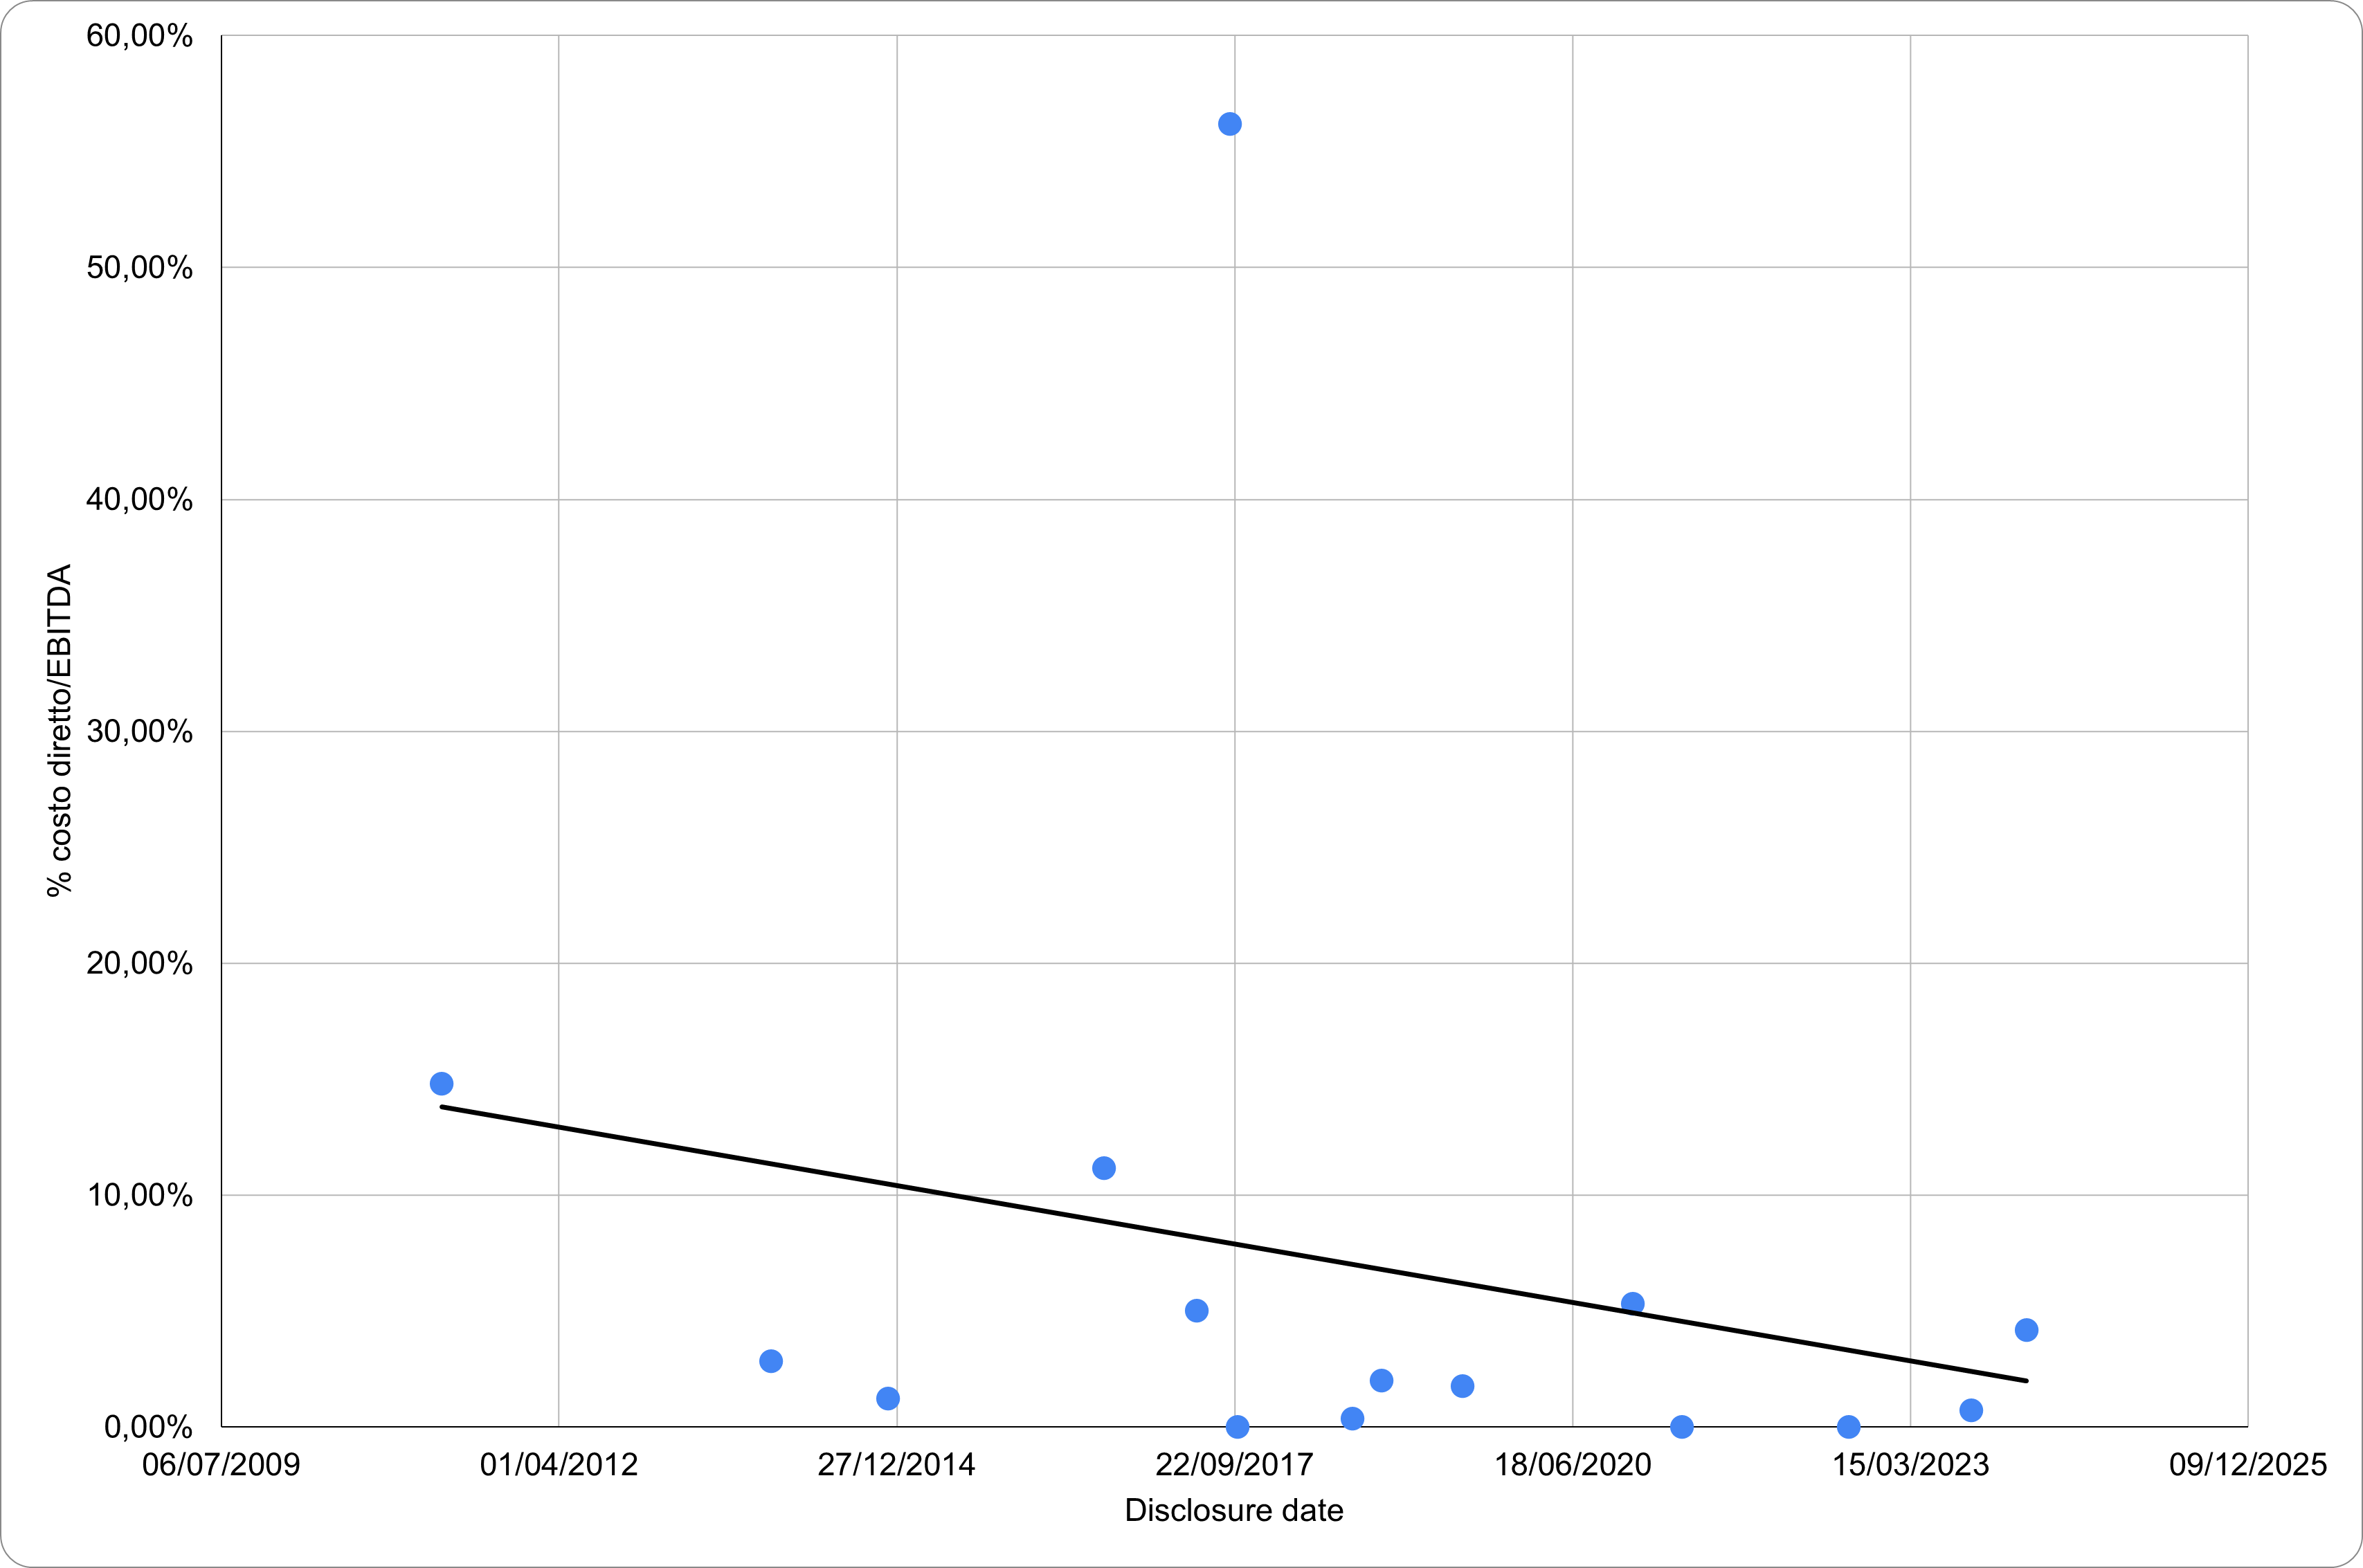
\includegraphics[width=1\linewidth]{figures/ebit-date-1.png}
        \caption{EBITDA nel tempo}
        \label{fig:ebit1}
    \end{subfigure}
    \begin{subfigure}{0.48\textwidth}
        \centering
    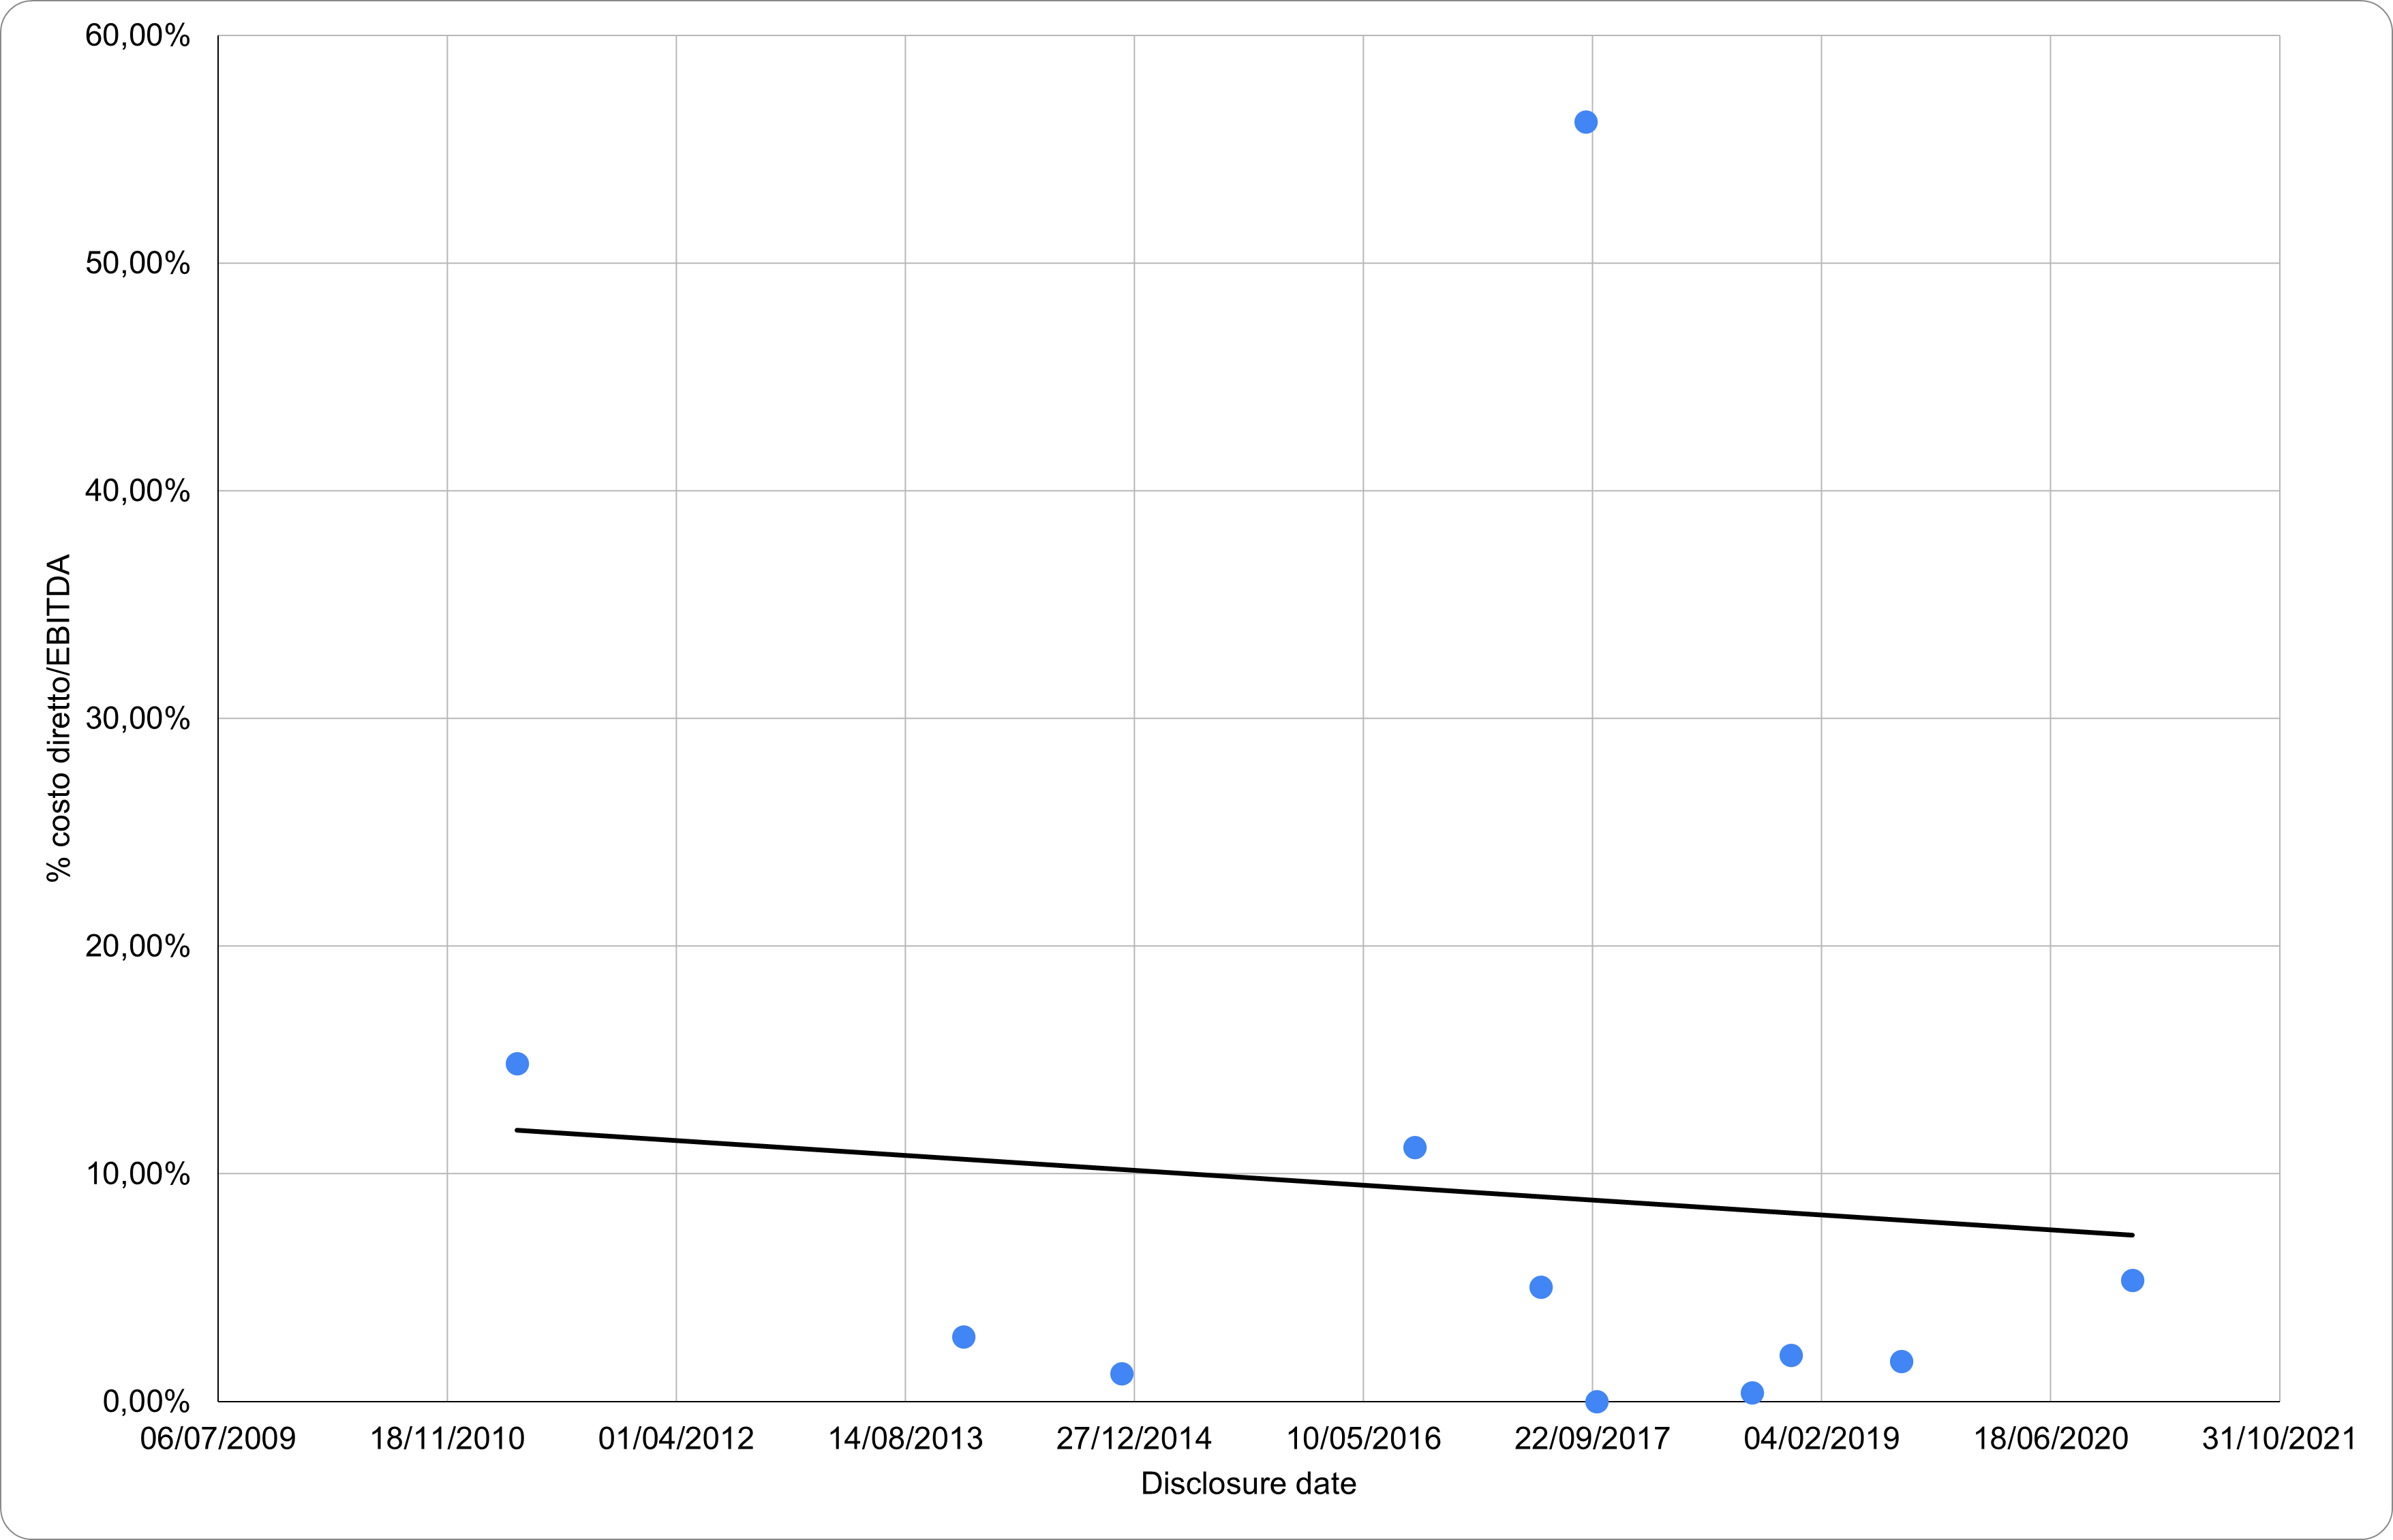
\includegraphics[width=1\linewidth]{figures/ebit-date-2.png}
    \caption{EBITDA nel tempo corretto}
    \label{fig:ebit2}
    \end{subfigure}
\end{figure}
Il trend discendente evidenzia un calo dei costi diretti in relazione alla redditivit\`a dell'azienda, che potrebbe derivare da una maggiore prontezza ed efficienza nella gestione sul piano tecnico da parte delle aziende di media-grande dimensione prese in esame nello studio.\\


\subsection{Azioni}
Quanto detto prima non si applica al percepito e alla reazione dei mercati finanziari secondo figura \ref{fig:stockloss}. Il trend crescente funge da monito e restituisce un quadro in cui la prevenzione rimane centrale nonostante il calo di costi diretti connessi agli attacchi.\\
\begin{figure}[H]
    \centering
    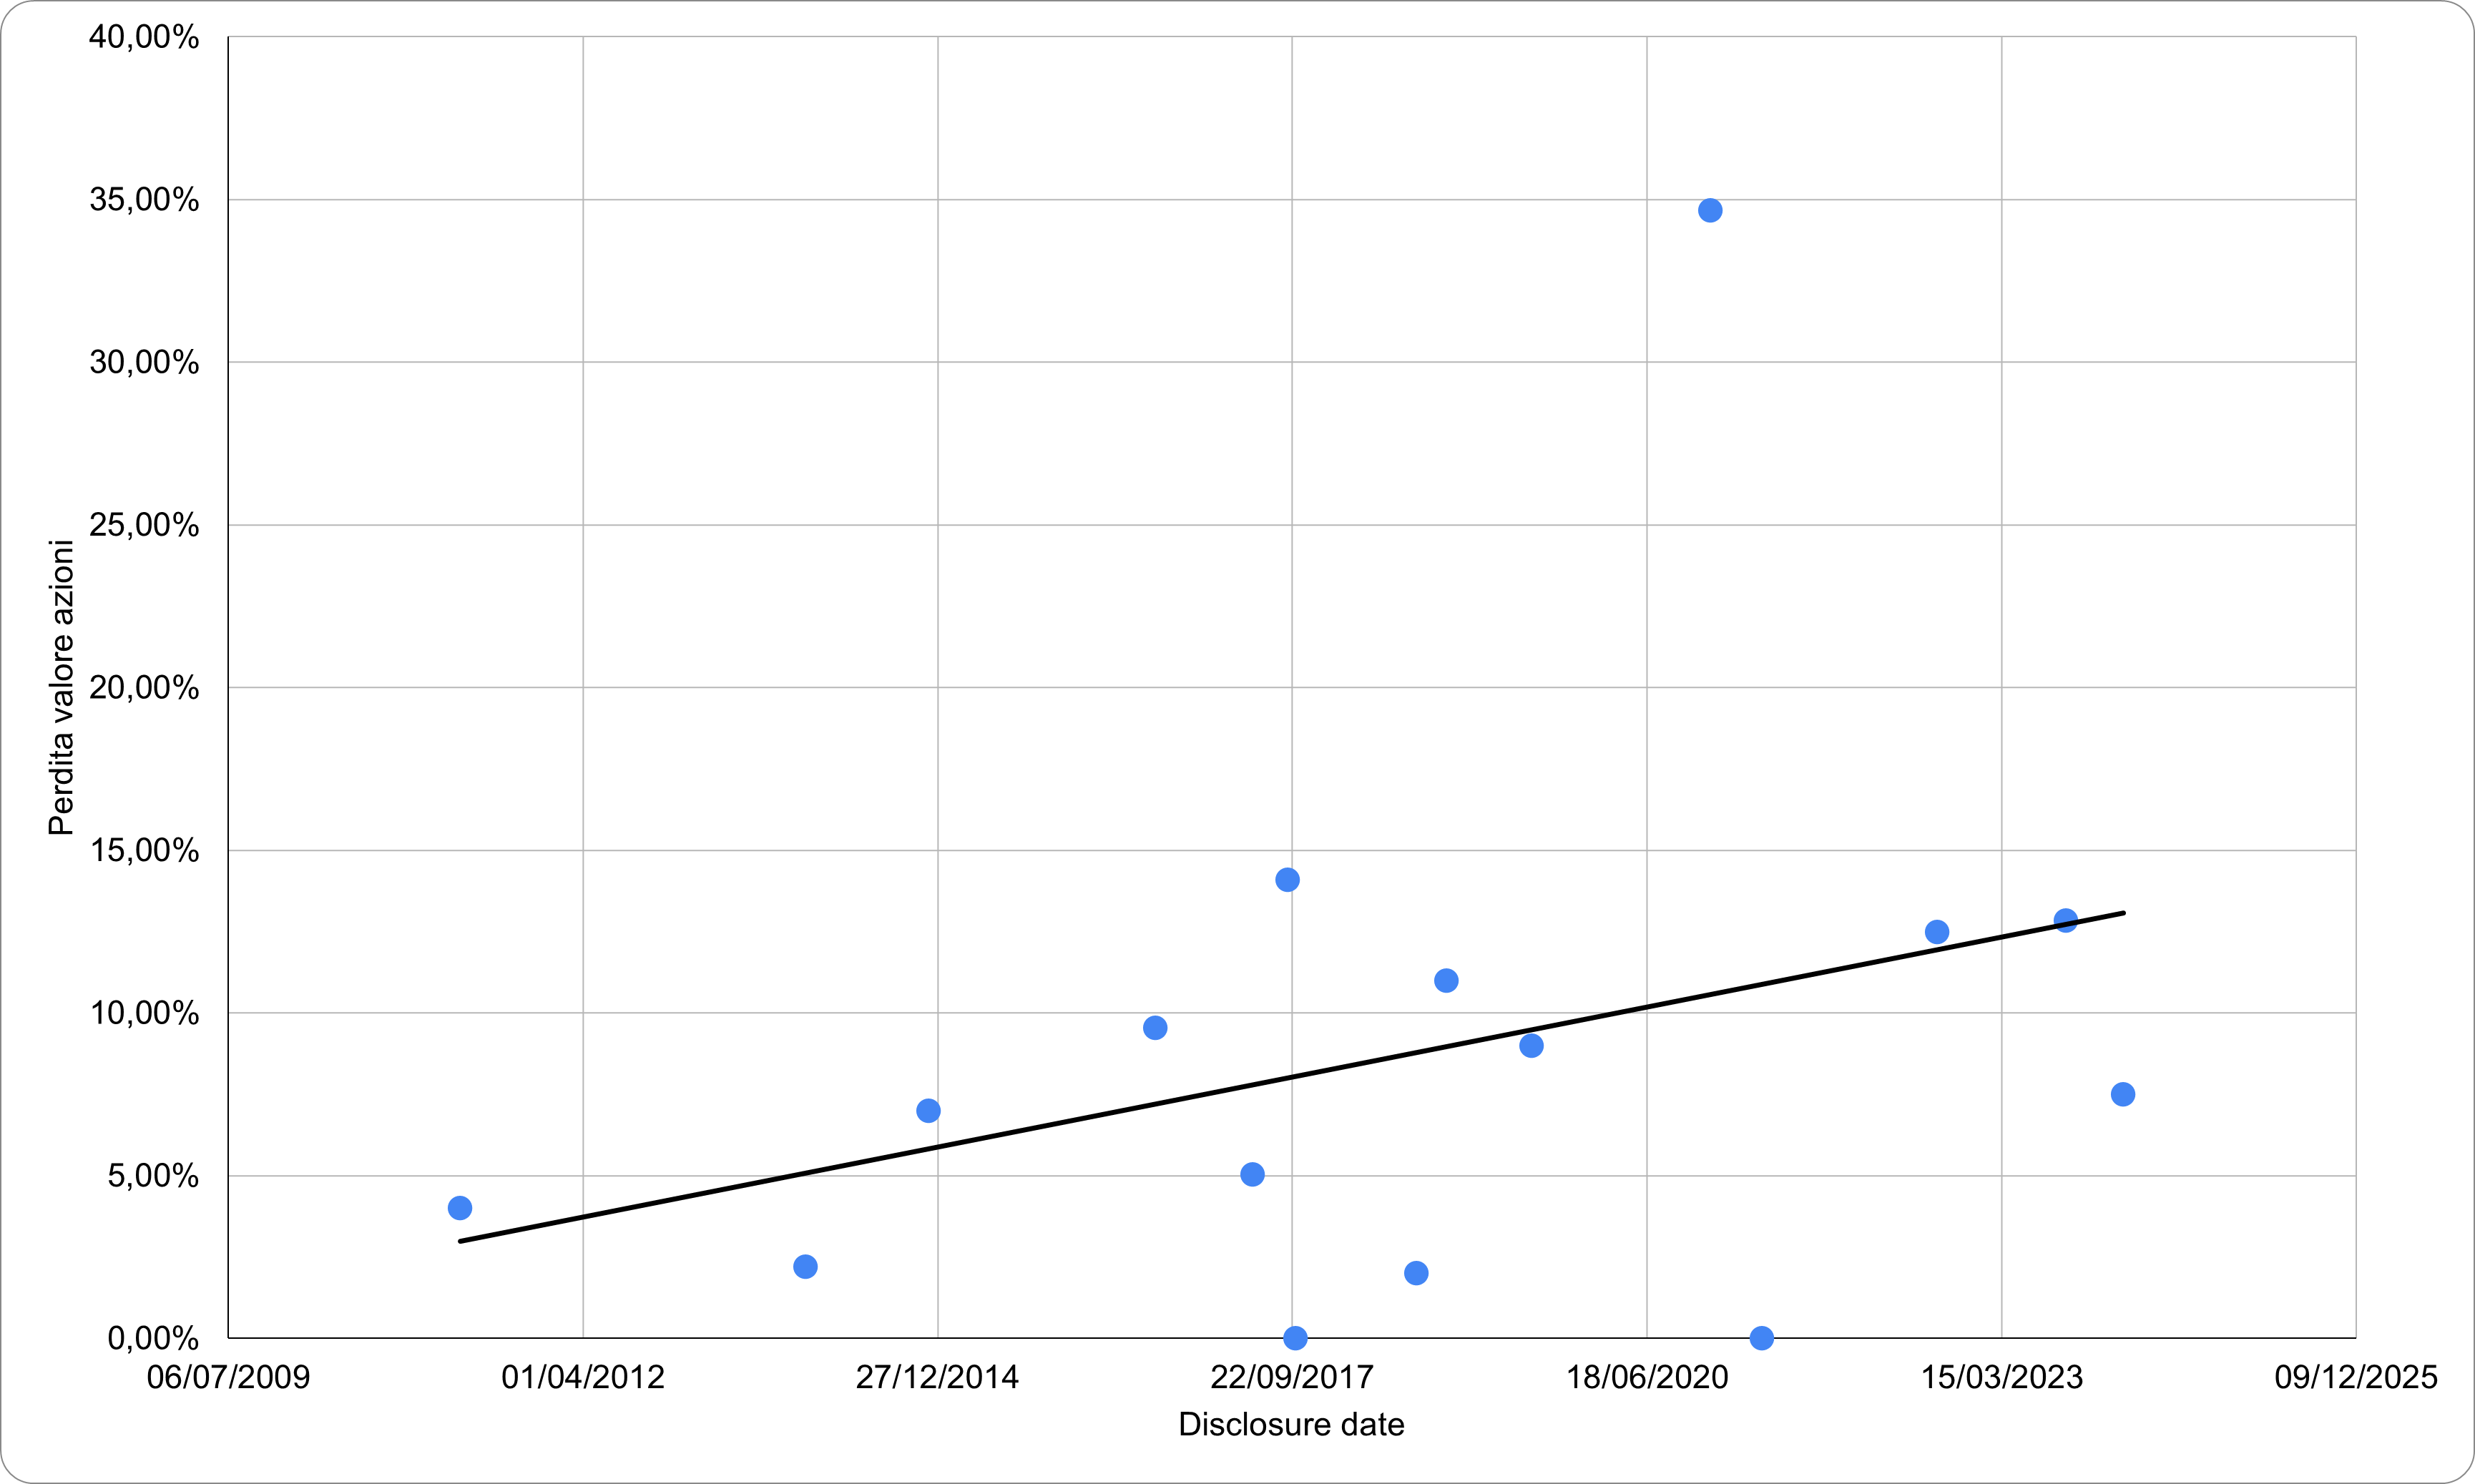
\includegraphics[width=10cm]{figures/stocks-date.png}
    \caption{Perdita di valore delle azioni a breve termine nel tempo}
    \label{fig:stockloss}
\end{figure}

\clearpage{\pagestyle{empty}\cleardoublepage}



%%%%%%%%%%%%%%%%%%%%%%%%%%%%%%%%%%%%%%%%
% CONCLUSIONI
\chapter{Conclusioni}

Lo studio evidenzia una controtendenza rispetto all'effettiva crescita del 
costo degli attacchi informatici menzionata precedentemente, una crescente 
propensione a crolli considerevoli nel valore di mercato e l'incremento
nel tempo del numero di attacchi \textit{ransomware}.\\
Sebbene una valutazione su un campione cos\`i ridotto sia esposta ad errori
\`e possibile interpretare questi dati come una minore propensione o 
minore efficacia degli hacker negli attacchi a grandi aziende che si
dimostrano sempre pi\`u preparate. Ma se comunque il costo complessivo 
\`e in fortissima crescita \cite{cybercrime_magazine} il risultato \`e 
un danno maggiore per enti collegati o un aumento del numero assoluto di
attacchi ad aziende pi\`u piccole che spesso non si interessano sufficientemente
 o non hanno i mezzi adeguati.\\
A fronte di ci\`o risulta evidentemente necessario potenziare per qualunque
azienda la propria copertura in ambito di sicurezza informatica.\\
\\
In italia, dove la maggioranza delle aziende sono piccole o medie imprese, 
sarebbero probabilmente efficaci degli incentivi statali che, aiutando lo 
sviluppo di un livello adeguato di protezione in maniera capillare,
permetterebbe di ridurre considerevolmente anche i danni agli enti connessi.


\clearpage{\pagestyle{empty}\cleardoublepage}



%%%%%%%%%%%%%%%%%%%%%%%%%%%%%%%%%%%%%%%%%
% BIBLIOGRAFIA
\rhead[\fancyplain{}{\bfseries Bibliografia}]
{\fancyplain{}{\bfseries\thepage}}
\addcontentsline{toc}{chapter}{Bibliografia}
\label{Bibliography}
\bibliographystyle{IEEEtran}
\bibliography{src/bibliography}

\end{document}